%!TEX root = ../thesis.tex
%*******************************************************************************
%****************************** Second Chapter *********************************
%*******************************************************************************

\chapter{Background}
\label{chapter background}

\ifpdf
    \graphicspath{{Chapter2/Figs/Raster/}{Chapter2/Figs/PDF/}{Chapter2/Figs/}}
\else
    \graphicspath{{Chapter2/Figs/Vector/}{Chapter2/Figs/}}
\fi

Measuring blood flow to the extremities provides valuable information to the clinical community. Being capable of estimating instant blood flow in a limb provide information on the health of the "highways" of oxygen and nutrient transport to these tissues via the vasculature. Some diseases cause problems with the micro or macro-vasculature. Some of these diseases include cardiovascular disease, peripheral vascular disease, diabetes and Raynauds syndrome. Without adequate blood flow these tissues will become ischaemic (\textit{isch} in Greek means to stop or block and \textit{emia} that means blood flow) and if severely compromised, necrosis (death of tissue) will ensue. In medicine, the clinician always tries to salvage tissue when able to. Therefore, measuring the disease progression or acute problems with the vasculature in the extremities can help clinicians decide how to proceed with the proper treatment which may include a bypass grapht or if unable to salvage, then amputation.

\rvmynote{This introduction needs to be improved. More about what I'm going to describe should be added}

The following chapter describes the importance of blood flow as well as the problems and complications derived from a poorly perfused limb. Following this, some of the current technologies used to estimate blood flow will be explained.  

\section{Circulatory system} %section 2.1
\label{section literature circulatory system}
The human body has a closed circulatory system, where the blood is enclosed within the blood vessels and is transported to and from the heart which works as a pump. The main function of the circulatory system is to carry oxygen and nutrients to all the cells in the body as well as collecting the by-product of the metabolic process. Blood flows through vessels that form a complex, elastic tubular network that reaches each cell of the body. The arteries carry oxygenated blood, and the veins return de-oxygenated blood. 

Blood moves from the arterial to venous circulation within the capillaries. Plasma passes through capillaries that are only a cell's thickness in diameter. After, an increase of blood pressure forces interstitial fluid out of the capillary walls. In the end, some of this fluid returns to the capillaries, and some go into the lymphatic vessels. The different components of the circulatory system will be described in more detail in the following sections. In particular, the anatomy of the arm will be explained in more depth as it is the part of the body that will be tested by the device designed.

%********************************** %Section 2.1.1 **************************************  
\subsection{The blood}
\label{section literature blood}
Blood is the main carrier of nutrients that run through humans and vertebrate animals. It also plays a significant role in the body's defence combating infections. In short, it is in charge of transporting oxygen and collecting carbon dioxide from all the tissues that constitute the body. Blood requires different paths to circulate in the human body; the circulatory system is used to carry oxygenated and deoxygenated blood, also known as arterial and venous blood respectively. Indeed, the body uses arteries to transport oxygenated blood coming out from the heart via the lungs and uses veins to return deoxygenated blood to the heart and back to the lungs.

%********************************** %Section 2.1.1.1  **************************************  
\subsubsection{The blood plasma}
It is important to describe the plasma as one of the main electrical conductors in the human body. The plasma is the suspending medium where the blood cells described by table \ref{table:cell} travel around the body. Indeed the extracellular fluids originate from the plasma's fluid.

The solutes inside the plasma play important roles at a cellular level. Within it, amino acids, glucose and vitamins are dissolved to be used by the cellular metabolic process. Additionally, there are hormones present that regulate the activity of blood cells and their activation also creates chemical by-products within the circulature such as nitrogen ($N$) and $CO_2$.

The plasma is mainly composed of salt and water. In fact, it is quite similar to seawater but with a lower concentration of ions. Some of the ions present in significant numbers are sodium ($Na$), chloride ($Cl^-$)and bicarbonate ($HCO_3^-$) ions. However, there are also traces of calcium, magnesium, copper, potassium and zinc.

Proteins are produced by the liver and are an essential component found in the plasma. The most common protein found in it is albumin, which serves as depot protein and transport protein, for instance, it bounds with long-chain fatty acids and bilirubin \cite{kragh1981molecular}. Besides, there are alpha and beta globulins that convey lipids and steroid hormones, and \textit{fibrinogen} used during the clotting process.

%********************************** %Section 2.1.1.2 **************************************  
\subsubsection{Blood cells}
There are well known and identifiable components in blood. Approximately, half of its volume consists of plasma, the properties of which were described previously. The other half of the blood is comprised of red blood cells (erythrocytes), white blood cells (leukocytes or monocytes) and platelets (thrombocytes). In short, the red blood cells function is to transport oxygen; the white blood cells are in charge of the immunological response, and platelets, the clotting process.

However, these cells also perform other specialised tasks. Their properties and characteristics are described more in detail in table \ref{table:cell}, it also includes cells quantity per microliter (\si{\micro\litre}) of human blood. It must be noted that there are diverse specialised subtypes of white cells and platelets but no further details of this will be explored in this work.

\begin{table}
\caption{Blood cell classification}
\label{table:cell}
\centering
\begin{tabular}{ >{\raggedright}p{0.18\textwidth}  
		         >{\raggedright}p{0.12\textwidth} 
		         p{0.22\textwidth} 
		         p{0.37\textwidth}}
\toprule
  \textbf{Cell Type }
& \textbf{Quantity} 
& \textbf{Geometry} 
& \textbf{Characteristic} \\
\midrule
	Red Blood Cells (RBCs) or erythrocytes 
	& \numrange{5e6}{6e6} 
	& Shape: Disk \newline Diameter: 6-\SI{8}{\micro\meter} \newline Thickness: \SI{2}{\micro\meter} 
	& \begin{tabular}[t]{P{0.34\textwidth}} 
	    \tabitem Principal medium to deliver oxygen \\
	    \tabitem Lack of nucleus \\
	    \tabitem Cytoplasm rich in negatively charged Iron–containing Hb \\
	    \tabitem Contains Ions of Sodium ($Na^+$) and Potassium ($K^+$) \\
	    \tabitem Typical bilayer lipid membrane (Lipid composition defies physical properties such as membrane permeability and fluidity) 
	  \end{tabular} \\
\midrule
	White Blood Cells (WBC) or Monocytes 
	& \numrange{4e3}{11e3} 
	& Shape: Irregular \newline Diameter: 10-\SI{20}{\micro\meter} \newline Monocytes: 14–17 
	& \begin{tabular}[t]{P{0.34\textwidth}} 
	    \tabitem Composed five different type of specialised cells to target different illnesses\\
	    \tabitem Make part of the immune system \\
	    \tabitem High count of these cells are indicators of disease 
	  \end{tabular} \\
\midrule
	Platelets 
	& \numrange{150e3}{400e3} 
	& Shape: Irregular \newline Diameter: 2–\SI{3}{\micro\meter}  
	& \begin{tabular}[t]{P{0.34\textwidth}}
	    \tabitem Lack of nucleus  \\
	    \tabitem Responsible for procoauglant activity \\
	    \tabitem If count to low excessive blood may occur. Too high blood cloth might form (thrombosis)
	  \end{tabular} \\ 
\bottomrule
\end{tabular}
\end{table}

\subsection{Blood vessels}
The blood leaves the heart through the arteries that reach all the organs of the body. This network of arteries branch into a microscopic size, at which point they are called arterioles. From here, blood enters the capillaries, which are tiny thin-walled tubes that reach the size of a cell. Venules collect the blood that comes out of the capillaries and then moves to the main veins, which carry it back to the heart.

Arteries, arterioles, veins and venules are composed of the same cellular structure (see figures \ref{fig:arteries composition} and \ref{fig:veins composition}). The innermost part of these vessels is an epithelial coating known as the endothelium. A thin layer of elastic fibres, a smooth muscle and connective tissue, lies around the endothelium. Capillaries are much thinner compared to these vessels. Indeed, capillaries are made only of endothelium cells which allow the exchange of fluids between the blood and the surrounding tissue (see figure \ref{fig:capillaries composition}). This interchange of molecules and ions between both occurs by diffusion, by filtration at the capillary walls, and by transport through endothelial cells. Hence, it is here where the exchange of gases and metabolites occurs between the blood and the body's cells \cite{johnson2001biology}.

\begin{figure*}[!htbp]
	\centering
	\begin{subfigure}[t]{0.33\textwidth}
		\centering
		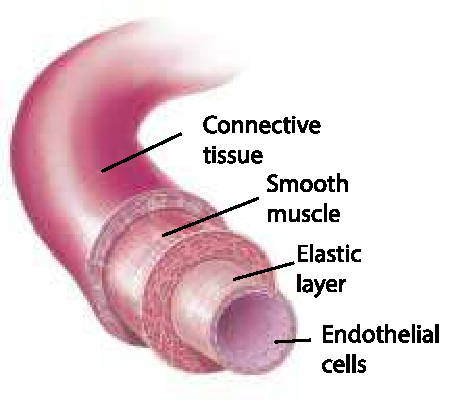
\includegraphics[width=5cm]{figure1a}
		\caption{Layers of the arteries}
		\label{fig:arteries composition}
	\end{subfigure}%
	~ 
	\begin{subfigure}[t]{0.33\textwidth}
		\centering
		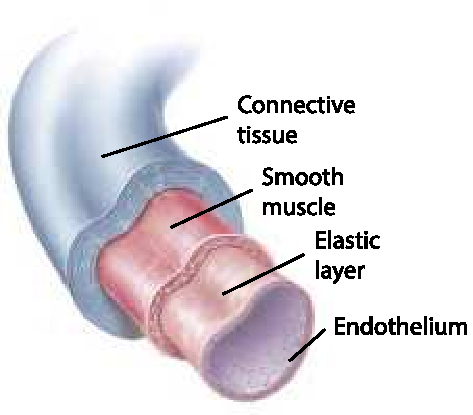
\includegraphics[width=5cm]{figure1c}
		\caption{Layers of the venous}
		\label{fig:veins composition}
	\end{subfigure}
	~ 
	\begin{subfigure}[t]{0.33\textwidth}
		\centering
		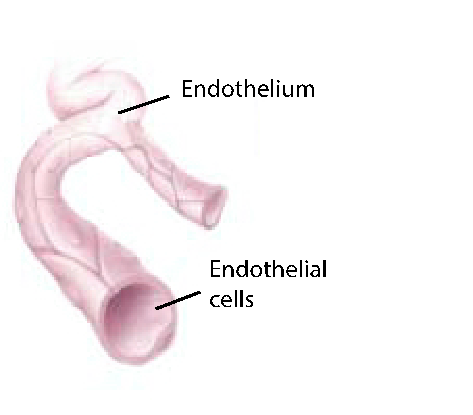
\includegraphics[width=5cm, trim={0 0 2cm 0},clip]{figure1b}
		\caption{Layers of the capillaries}
		\label{fig:capillaries composition}
	\end{subfigure}
	\caption[Layers of the blood vessels]{The arteries and veins have the same kind of layers. However, the smooth muscle is thicker in arteries than veins. The capillaries have a thin wall and are composed only by endothelium. Figure adapted from \cite{johnson2001biology}.}
	\label{fig:vessels composition}
\end{figure*}

\subsubsection{Arteries and arterioles}
The arteries slightly differ from the arterioles in their composition. The main arteries contain additional elastic fibres within them, enabling greater compliance while receiving blood coming out the heart. On the other hand, smaller arteries and arterioles contain a thicker smooth muscle layer in their tunica media allow them to resist bursting.  

There is a direct relation between the diameter of the vessel and the frictional resistance to blood flow. The resistance to blood flow is inversely proportional to the radius of the vessel. Halving the diameter of a blood vessel increases 16 times its frictional resistance. Hence, the greatest resistance to blood flow in this branch of the circulatory system occurs in the small arteries and arterioles. Moreover, when the smooth muscle layer of the arterioles contracts, it produces vasoconstriction, which increases resistance and decreases blood flow. On the other hand, when this muscle relaxes vasodilation occurs, dropping resistance and increasing blood flow. Local chemical factors, the sympathetic system or hormones can control both muscle activities. Furthermore, blood flow towards some organs can also be regulated by precapillary sphincters. These rings of smooth muscle can shut down capillary beds totally. For instance, in cold weather, these precapillary sphincters may close to contribute to the vasoconstriction limiting heat loss.  

\subsubsection{Capillaries}
As previously described, the capillaries are considerably smaller than the rest of the blood vessels. On average, every one of them is about \SI{1}{\milli\meter} long and \SI{8}{\micro\meter} diameter, just big enough to allow a single red blood cell (RBC) (\SIrange{6}{8}{\micro\meter}) pass through. The capillary tree is so dense and extensive that every cell in the human body is within \SI{100}{\micro\meter} of reach.  Due to the enormous amount of them and their intricate network,  they have the greatest cross-sectional area of any other kind of blood vessel. Therefore, the blood decreases its velocity allowing more time to exchange metabolites with the surrounding extracellular fluid. As soon as the blood has left the capillary, all the exchange of $O_2$, nutrients, $CO_2$ and waste products has taken place. 

It must be noted, that the heart must produce enough pressure to overcome the resistance of the blood passing the arterial tree into the capillaries. However, blood loses most of its pressure when moving through the capillary network but also passes to a low-pressure system when entering to the veins. 

\subsubsection{Venules and veins}
Venules collect the blood that leaves the capillaries which then is deposited in the larger veins that lead the blood back to the heart. Due to the pressure in the venous return being one-tenth that of the arteries, venules and veins contain a thinner layer of smooth muscle. This pressure gradient also helps the blood to pass through the narrow passages of the capillaries. Most of the blood volume is contained within the veins, which also have the ability to expand to increase the body's blood capacity if needed. In order to help the blood return from the extremities, the surrounding skeletal muscle contracts by compressing the veins and pushing the blood back to the heart. Additionally, the veins contain valves that only allow blood to flow in one direction. However, a failure of any of these valves may lead to vascular problems such as varicose veins. 

\begin{figure}[!htpb]
	\centering
	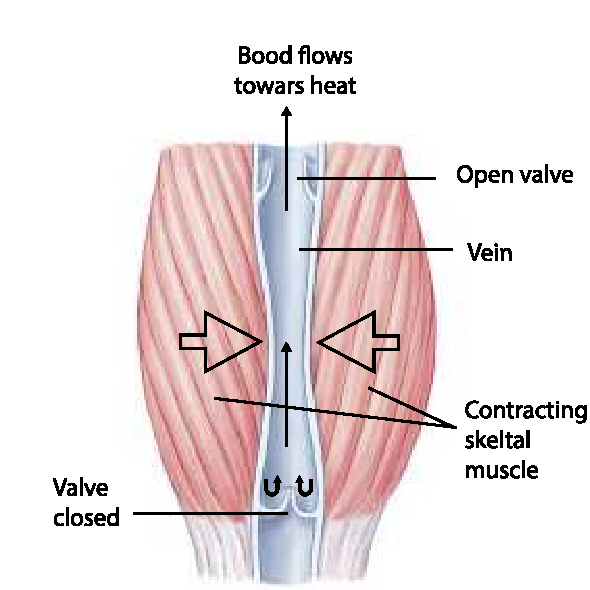
\includegraphics[width=0.5\textwidth,keepaspectratio]{figure2}    
	\caption[Venous return through skeletal muscle]{The vein only flows in on direction helped by valves along the vessel. Skeletal muscle contraction aids the return of blood to the heart. Figure adapted from \cite{johnson2001biology}. }
	\label{fig:venous return}
\end{figure}

\section{Cardiac cycle}
\label{background cardiac cycle}
It is important to understand how the heart operates because changes of volume are synchronous to the heart beating. As part of the circulatory cycle, the heart has to overcome the pressure of pushing RBC's through the capillaries. Hence, the heart has to work as a dual pump, pushing out arterial and collecting venous blood. The cardiac cycle is a periodic task that starts at the beginning of one heart beat until the start of the following one. The cycle is divided into ventricular contraction known as systole and ventricular relaxation called diastole. 

Each cardiac cycle is subdivided into phases where the heart experiences intense pressure change at a constant volume or a volume change with a minor alteration in pressure. During the systolic cycle the heart experiences (1) isovolumetric contraction followed by (2) blood ejection. On the other hand, diastole cycle follows the following steps (1) isovolumetric relaxation, (2) early diastolic filling,(3) slow ventricular filling (diastasis) and (4) atrial filling \cite{fukuta2008cardiac}. The heart rate is inversely proportional to the cardiac cycle and changes according to the body's needs. An average heart rate is about 75 beats per minute, where a single beat last around \SI{0.8}{\second}.

At rest, the duration of the systolic cycle takes about 1/3 of the total heart cycle and the diastolic cycle 2/3. When there is a high heart rate, as during exercise, this rate proportion changes, the duration of diastole takes much less time than during systole. The following sections will describe the changes in the heart, as well as pressures, electrical activity and heart sounds all along each cycle.

\begin{figure}[!htpb]
	\centering
	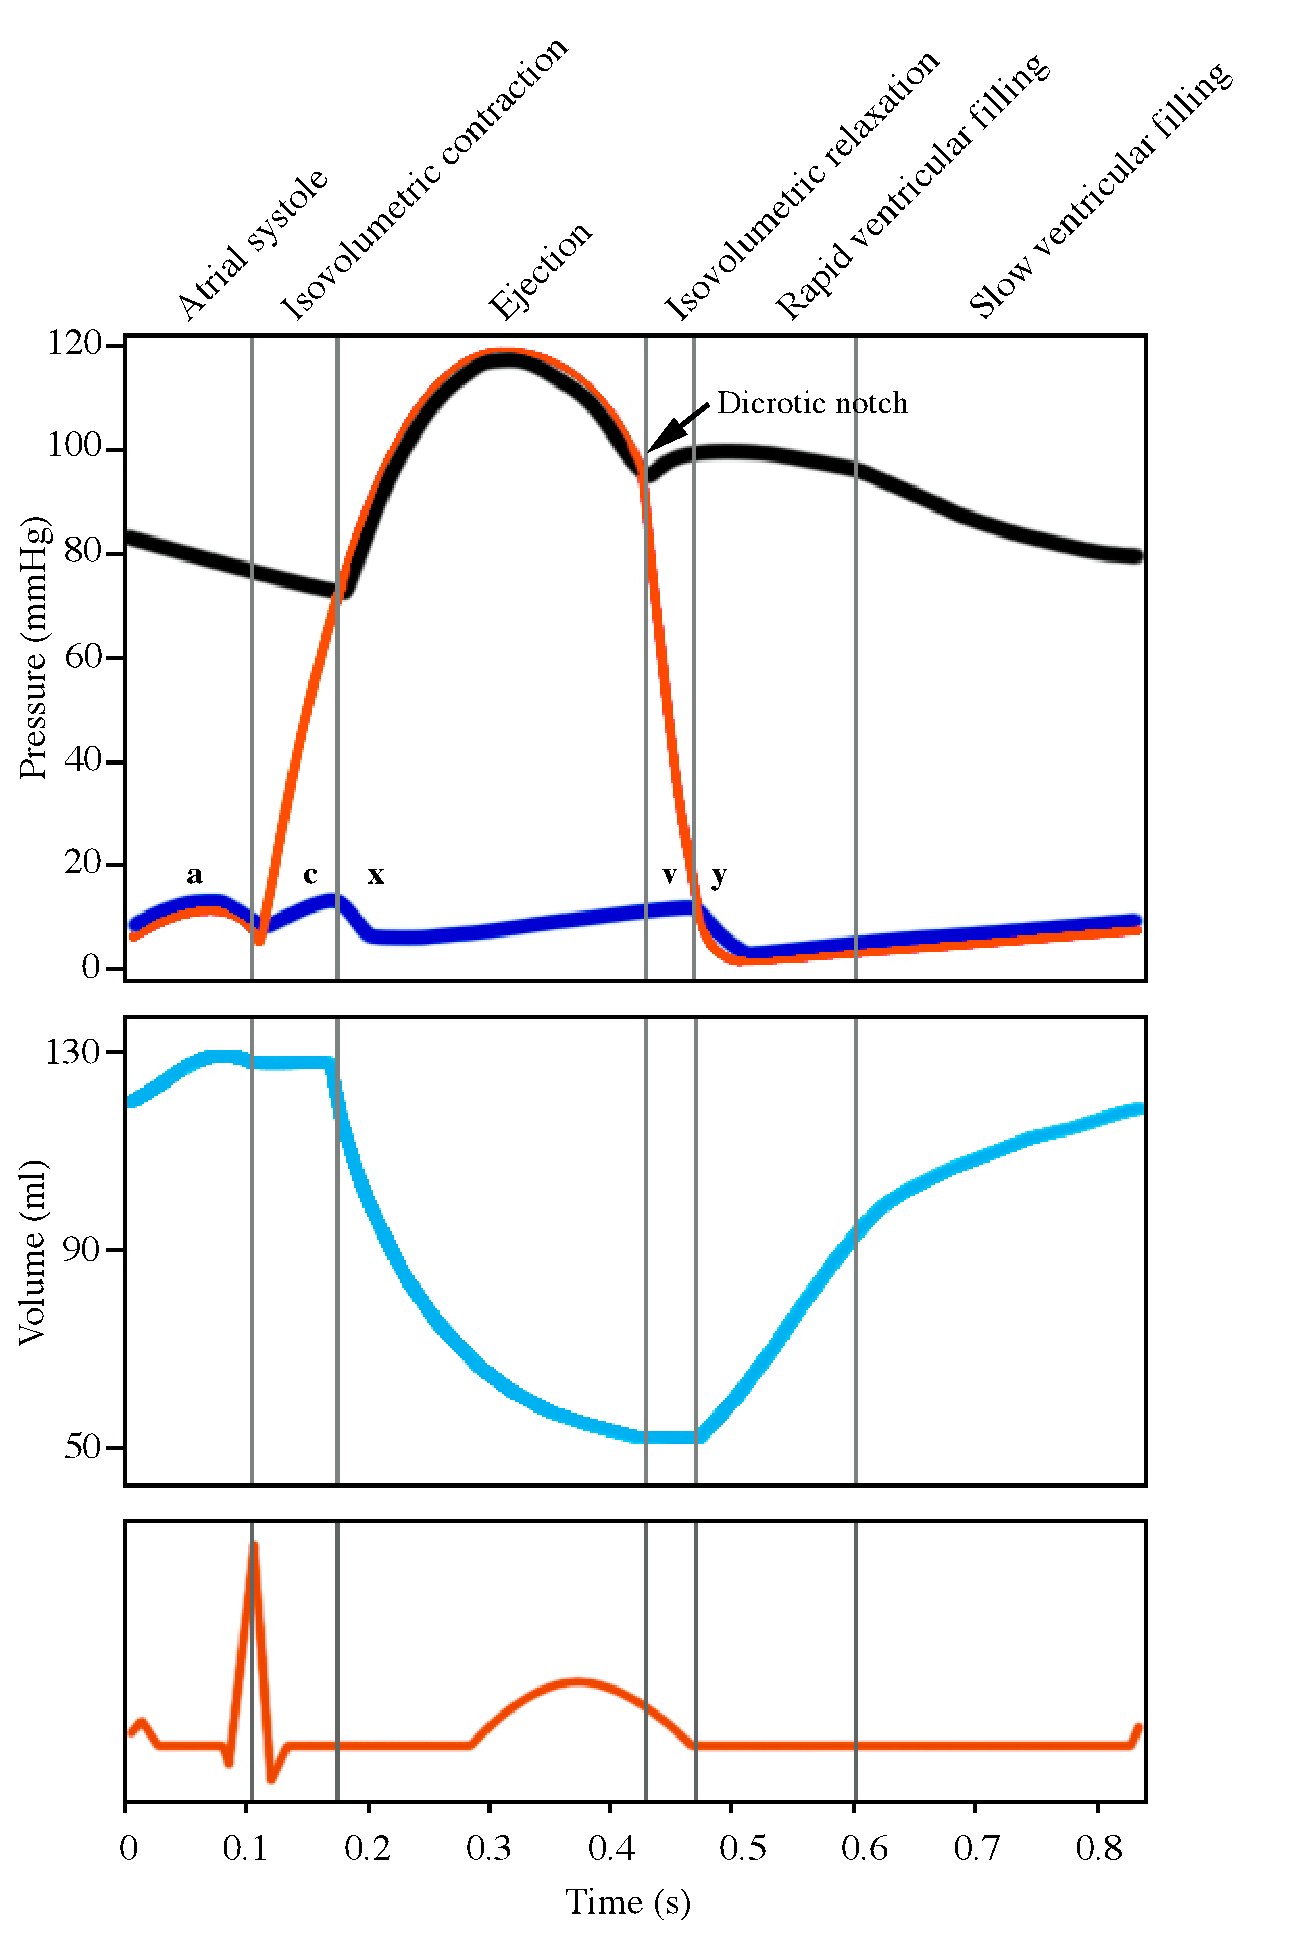
\includegraphics[width=8.5cm,keepaspectratio]{figure_pressure}    
	\caption[Changes of Pressure and Volume in the heart - ECG]{Pressures, volume changes and ECG changes during one hearth cycle. During the systolic cycle the heart experiences (1) isovolumetric contraction followed by (2) blood ejection. On the other hand, diastole cycle follows the following steps (1) isovolumetric relaxation, (2) early diastolic filling,(3) slow ventricular filling (diastasis) and (4) atrial filling \cite{fukuta2008cardiac}}
	\label{fig:heart cycle}
\end{figure}

\subsection{Systole}
\subsubsection{Isovolumetric contraction}
The etymology of the word isovolumetric comes from the ancient Greek, the prefix \textit{isos} meaning equal and \textit{volumetric} to reference volume. Hence, the in this cycle the heart keeps the same blood volume while the ventricles contract.

\begin{figure}[!htpb]
		\centering
		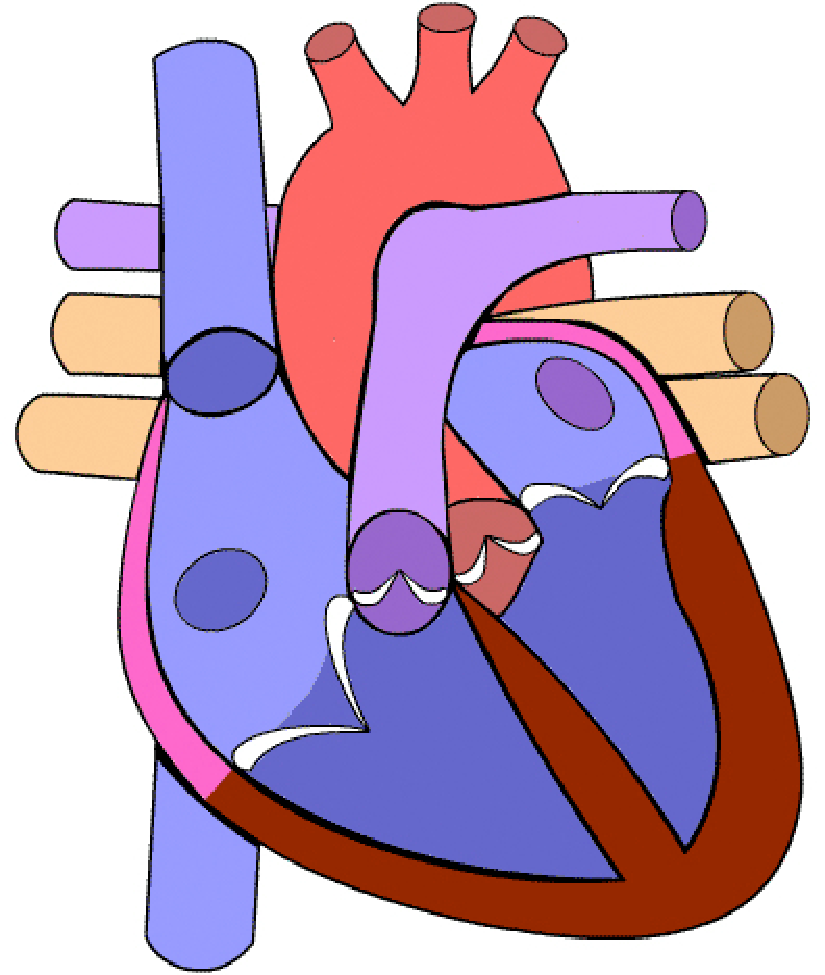
\includegraphics[height=4cm,keepaspectratio]{figure_3}   
		\caption[Heart during isovolumetric contaction]{Cross section of the heart during isovolumetric contraction. The contracted area is represented by the red colour.}
		\label{fig:heart isovolumic}
\end{figure}

Figure \ref{fig:heart cycle} shows the variation of pressure in the left ventricle, the right atrium, the aortic pressure and the ventricular volume. As the valves are shut, and the ventricles are contracted and blood can not leave the heart, the ventricular pressure increases but there is no change in the blood's volume. In the end, the total volume inside the ventricles is equivalent to the end-diastolic volume (about \SI{130}{\milli\litre}. In the atria, due to the differential of pressure between chambers the atrioventricular bulges backwards. Therefore, this valve change causes a small variation of pressure in the right atrium. It is depicted as the point c in the same figure. The pressure in the systemic and pulmonary arteries drops at a constant rate. 

\rvmynote{I need to reference this to the website or a book.}

The electrocardiogram waveform shown in figure \ref{fig:heart cycle} displays the electrical activity of the heart during this section of the cycle. In short, the depolarization of the heart starts from the atrioventricular node spreading through the bundle of His and Purkinje fibres to the septum and the walls of both ventricles. This event causes the QRS complex shown in the same figure. At the same time, the atrial repolarisation causes the atrial T wave which is not visible in the ECG because the QRS complex covers it.

\rvmynote{Add a reference to this text from a medical book.}

%\begin{figure}[!htpb]
%	\centering
%	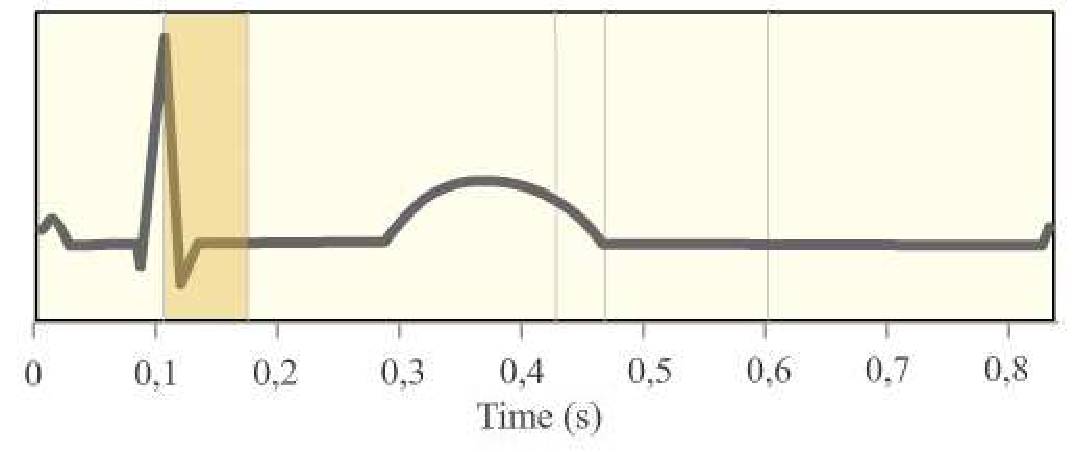
\includegraphics[width=0.5\textwidth,keepaspectratio]{figure_5}    
%	\caption[Isovolumic contraction - ECG]{ECG during isovolumic contraction.}
%	\label{fig:ECG isovolumic}
%\end{figure}

\subsubsection{Ejection}
During this cycle, the mechanics of the heart experiences the following changes. The gradient of pressure is greater in the left ventricle compared that of the aorta. The increasing pressure of the right ventricle exceeds that of the pulmonary artery. Hence, causing the semilunar valves to open. Due to the ventricular contraction, the blood is ejected from both ventricles to the aorta and pulmonary arteries and the atrioventricular valves are closed.

\begin{figure}[!htpb]
	\centering
	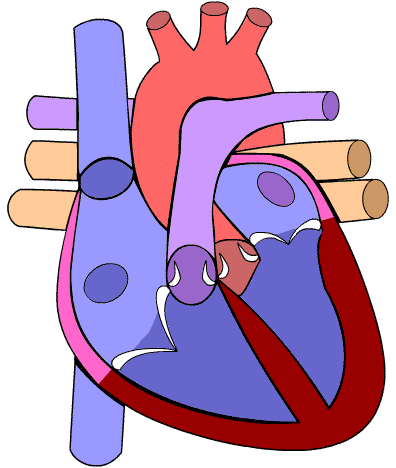
\includegraphics[height=4cm,keepaspectratio]{figure_6}
	\caption[Cross section of the heart during the ejection cycle]{Cross section of the heart during the ejection cycle. The contracted area is represented by the red colour. The semilunar valves are open.}
	\label{fig:heart ejection}
\end{figure}

To explore this in more detail, this cycle divides itself into a rapid and slow ejection. Regarding pressure, the increasing ventricular pressure during the contraction creates the sudden purge of blood toward the arteries. Then, the blood volume within the ventricles and arteries begins to drop. Due to the pressure difference between these two, the blood is ejected slowly. During this cycle, normally the maximum pressure of the left ventricule reaches about \SI{120}{\mmHg}, which is known as systolic pressure and \SI{25}{\mmHg} in the right ventricle. These pressures are also transferred to the aorta and pulmonary arteries respectively which also start to drop after reaching these peaks. Regarding blood volume, under normal conditions while resting only \SI{70}{\milli\litre} of blood is ejected, this is known as the stroke or systolic volume. The rest \SI{60}{\milli\litre} remains in the heart until the end of the cycle which is known as end-systolic volume. The relation between stroke volume and the end-diastolic volume is known as ejection fraction, of which \SI{60}{\percent} being the normal physiological range. The atria also contract during this cycle. The pressure in the atria and main vein vessels decreases because they are being elongated by the shortening of the ventricles. Hence, there is a drop in the atria's pressure. 

From the electrical point of view, at the beginning of this cycle, the ventricles are completely depolarised which is equivalent to the ST segment of the electrocardiogram. Due to ventricular repolarisation, the T wave can be seen in the second part of this stage. 

\subsection{Diastole}
\subsubsection{Isovolumetric relaxation}
In the heart's mechanics, once the heart completes its systole the ventricles relax, and the pressure starts to drop rapidly. Then, due to blood inertia for a short period the blood flows out of the ventricles. The elevated pressures in the aorta and pulmonary arteries pushes back a little bit of blood towards the ventricle, which also causes the closure of the semilunar valves. Additionally, the atrioventricular valves are closed because the pressure in the atria is lower than that of the ventricle.

\begin{figure}[!htpb]
		\centering
		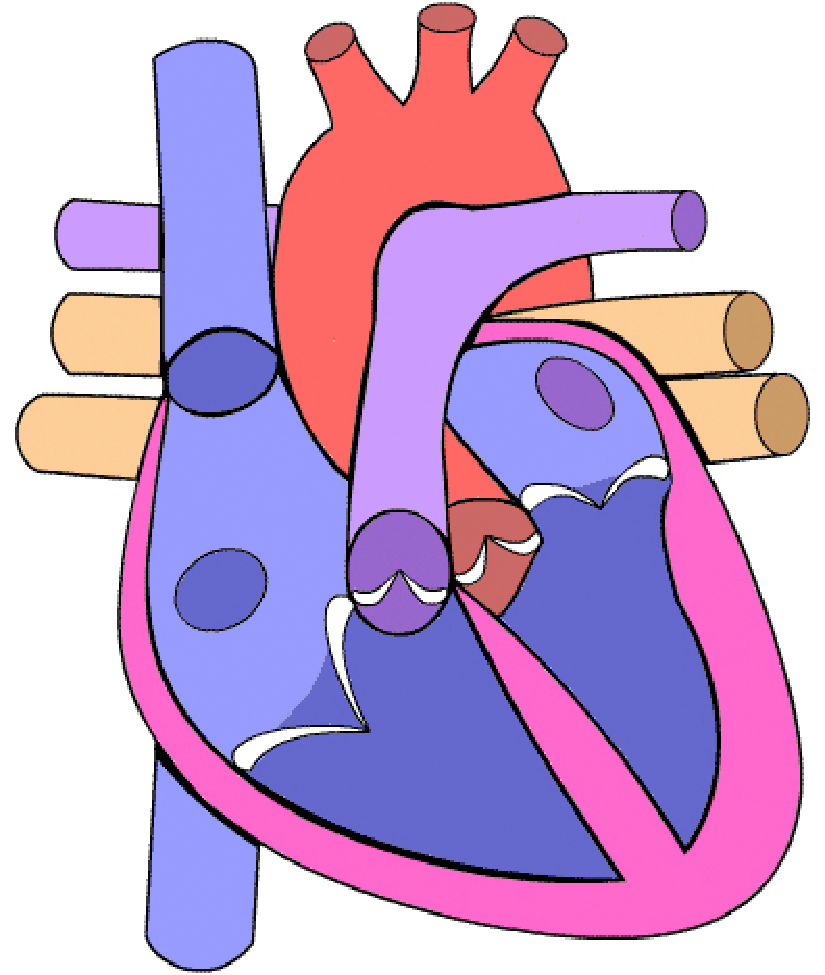
\includegraphics[height=4cm,keepaspectratio]{figure_9}
		\caption[Heart during isovolumetric relaxation cycle]{Cross section of the heart during the isovolumetric relaxation cycle. Semilunar and atrioventricular valves are closed in this stage.}
		\label{fig:heart isovolumetric relaxation}
\end{figure}

The changes of pressures and volumes in the different chambers occurs as follows. The ventricles relax rapidly, decreasing their pressure without altering the blood volume. Hence the name isovolumetric relaxation. Indeed, the blood remaining within the ventricle is still the end-systolic volume (\SI{60}{\milli\litre}. This relaxation period also causes a great drop in ventricular pressure until getting close to zero in both ventricles at the end of this cycle. The atria are filled with blood from the veins while the atrioventricular valves remain closed. This action increases the pressure in the atria (v wave in the plot). In the arteries, the decrease of their pressure is interrupted by the dicrotic notch which is a temporary increase in pressure that also creates a blood backflow which also closes the semilunar valves. 

During this period, the ventricle is completely repolarised completing the T wave in the ECG as shown in the figure.

\subsubsection{Rapid ventricular filling}
During this cycle, the ventricular pressure reaches a point where it is lower than the atrial one. Therefore, the atrioventricular valves open, allowing the blood accumulated in the atria to pass quickly into the ventricles. Most of the ventricular filling occurs during this stage. Furthermore, the blood volume within the ventricle increases but its pressure changes insignificantly due to the muscle relaxation. In the atria, there is a decrease in pressure (seen as venous pulse y wave) caused by the blood rushing out from the atria to the ventricles. 

\begin{figure}[!htpb]
	\centering
	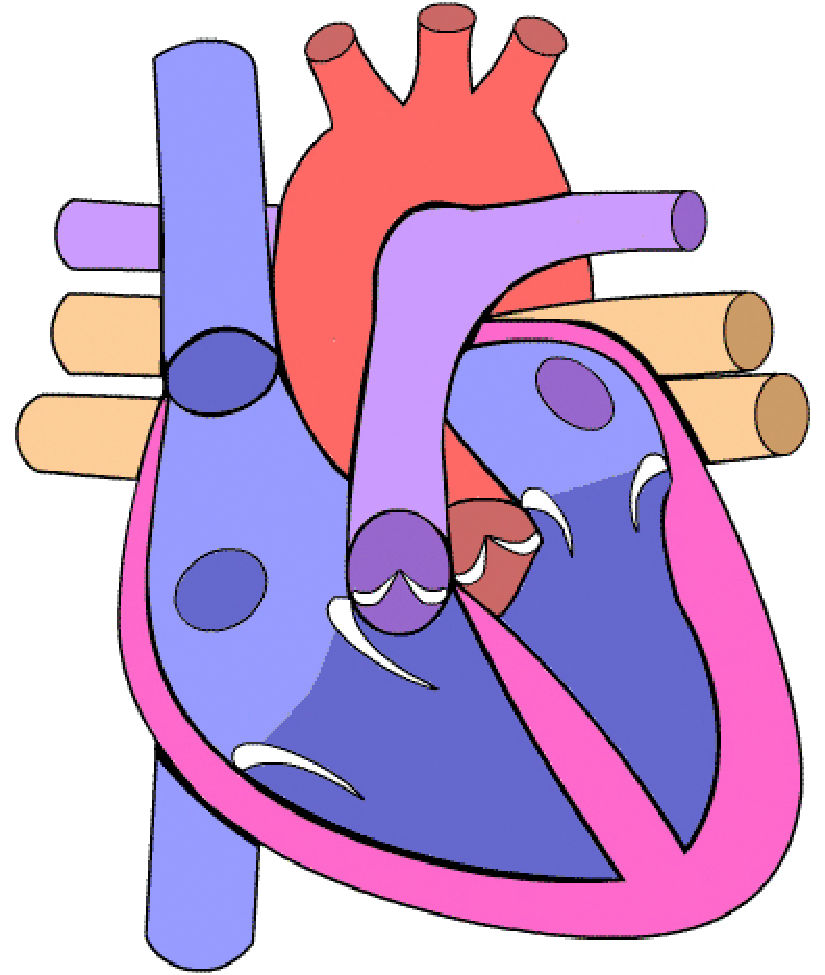
\includegraphics[height=4cm,keepaspectratio]{figure_12}
	\caption[Heart during rapid ventricular filling]{During rapid ventricular filling the atrioventricular valves open allowing blood to pass from the atria to the ventricles rapidly. The semilunar valves remain closed.}
	\label{fig:heart rapid ventricular filling}
\end{figure}

The semilunar valves stay closed during this stage, but the arterial pressure starts to decrease slowly. In the arteries, the blood pressure never goes to zero as it does in the heart because of their recoil properties. Indeed, the minimum arterial pressure in the systemic circulation during a heart beat is commonly \SI{80}{\mmHg} which is known as the diastolic pressure. In contrast, in the pulmonary circulation, the pressure could drop up to \SI{8}{\mmHg}. The electrical activity of the heart is null during this cycle. Hence, the isoelectric representation in the ECG wave.

%\begin{figure}[!htpb]
%	\centering
%	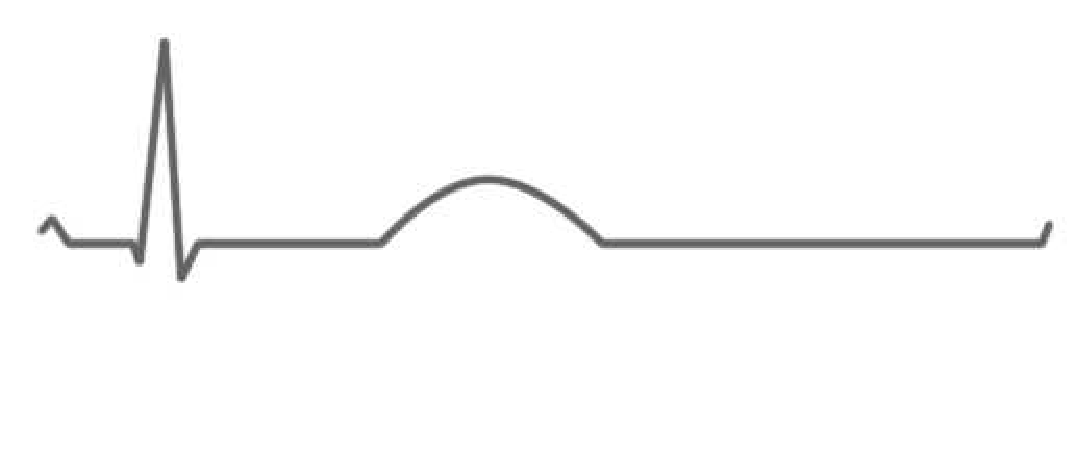
\includegraphics[width=0.5\textwidth,keepaspectratio]{figure_14} 
%	\caption[ECG during rapid ventricular filling]{During rapid ventricular filling there is not electrical activity.}
%	\label{fig:ECG rapid ventricular filling}
%\end{figure}

\subsubsection{Slow ventricular filling}
In this stage, there is no change in the mechanical activity of the heart. Certainly, the valves remain the same as in the rapid ventricle cycle. The atrioventricular valves are open and the semilunars closed. A small volume of blood flows into the ventricles, which come from the veins passing the atria and filling the ventricle slowly. The pressure in the ventricles still continues at zero, while the pressure in the atria slightly increases. Meanwhile, the pressure in systemic and pulmonary circulation drops at a constant rate. 

In the heart's electrical path, at the end of the cycle, the sino-atrial node depolarises and the electrical activity follows its course all around the heart producing the p wave showed in the ECG plot.  

%\begin{figure}[!htpb]
%	 \begin{subfigure}[t]{0.48\textwidth}
%	 	\centering
%	 	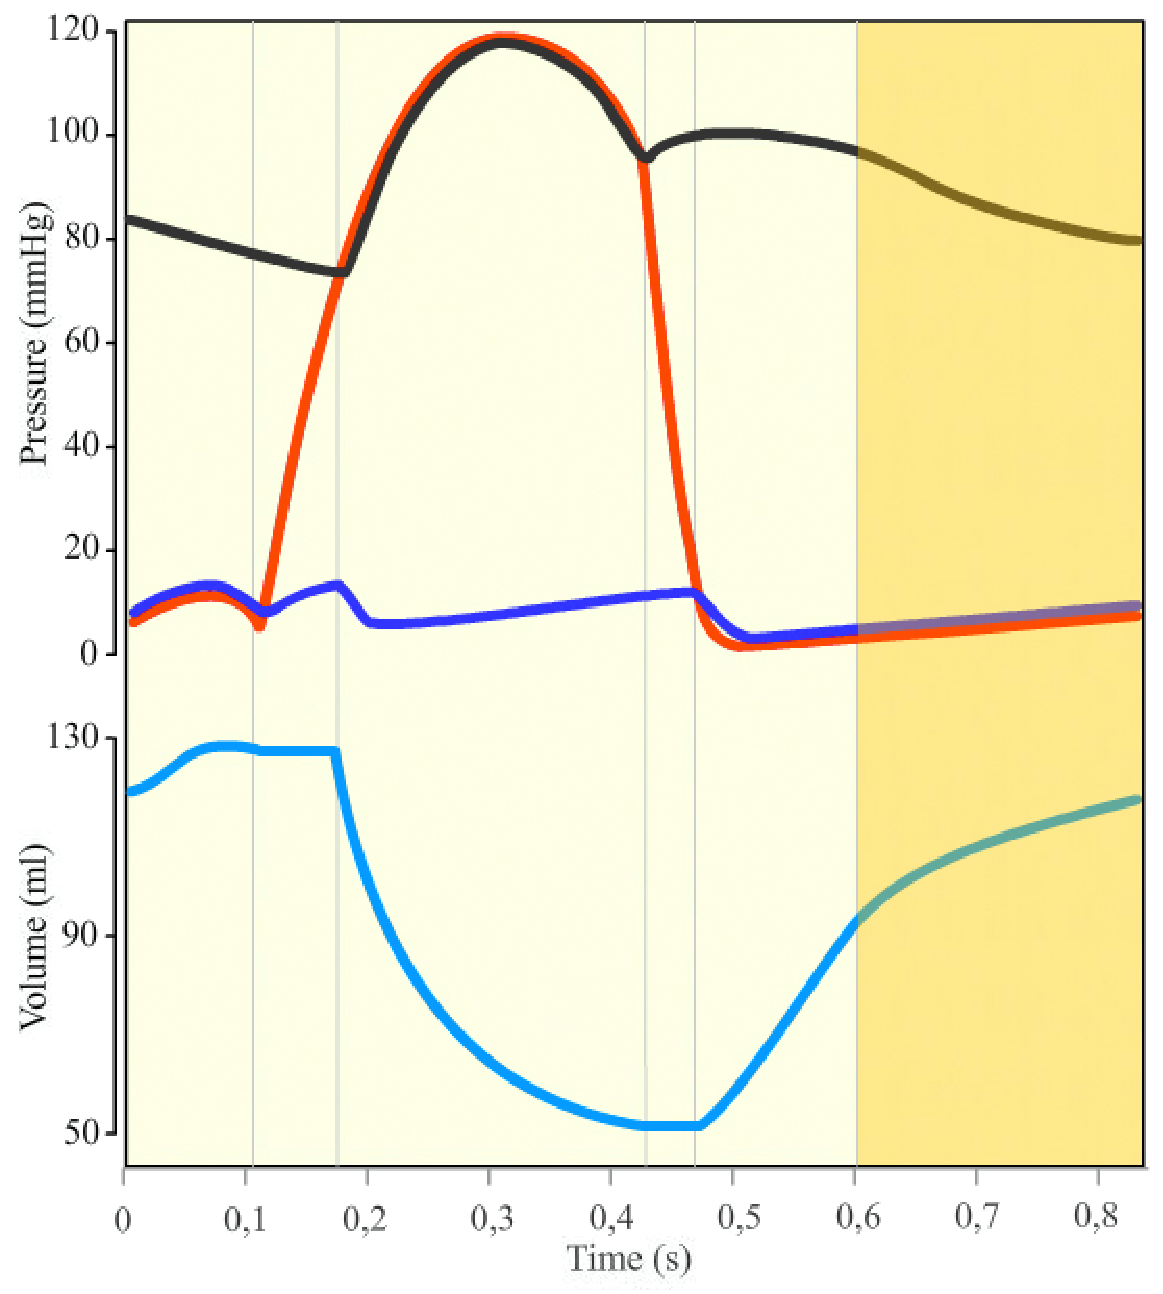
\includegraphics[width=\textwidth,keepaspectratio]{figure_15}
%	 	\caption{Ventricular pressure continues almost in zero (red line). The arterial pressure slowly decreases (black line), as well as the atrial pressure (dark blue). The blood volume in the ventricles (light blue) fill slowly.}
%	 	\label{fig:heart slow ventricular filling}
%	 \end{subfigure}
%	 ~
%	 \begin{subfigure}[t]{0.48\textwidth}
%	 	\centering
%	 	\raisebox{2.75cm}{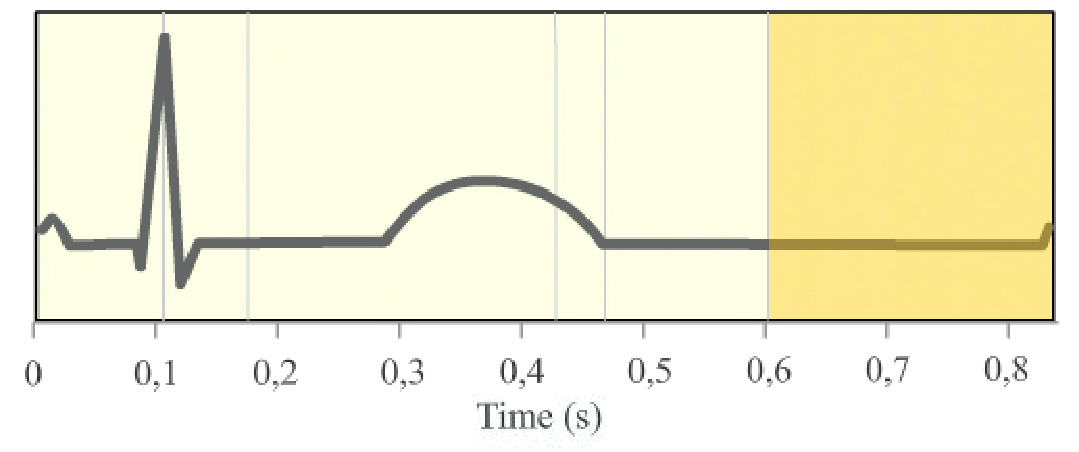
\includegraphics[width=\textwidth,keepaspectratio]{figure_16}}
%	 	\caption{The depolarization of the heart spreads from the sino-atrial node. The P wave is visible in the waveform. }
%	 	\label{fig:pressure slow ventricular fillig}
%	 \end{subfigure}
%	 \caption[Slow ventricular filling]{Pressures and volume during slow ventricular filling and ECG changes}
%\end{figure}
 
\subsubsection{Atrial systole}
Atrial systole is the last part of the cardiac cycle. In the mechanics of the heart during this phase, the ventricles fill entirely, while the atrioventricular valves open and the semilunar valves close. Additionally, an atrial contraction ejects blood from the atria to the ventricles. 

Thus, the atria eject approximately \SI{25}{\percent} of the ventricular filling volume to the ventricles. After that, the ventricular myocardium relaxes causing a slight change of pressure in the ventricles, remaining close to zero. At the end of the atrial systole, the total blood volume in the ventricles at the end-diastolic volume is about \SI{130}{\mmHg}. Due to the atrial contraction, there is a rise in pressure of these chambers. This can be seen as wave \textbf{a} in the venous pulse in figure \ref{fig:heart cycle}. Finally, the arteries pressure continues decreasing constantly.

The P wave of the ECG trace in figure \ref{fig:heart cycle} represents the moment atrial depolarisation occurs. Subsequently, the depolarisation spreads from the atria to the atrioventricular node which is portrayed by the PR segment in the ECG.

\begin{figure}[!htpb]
		\centering
		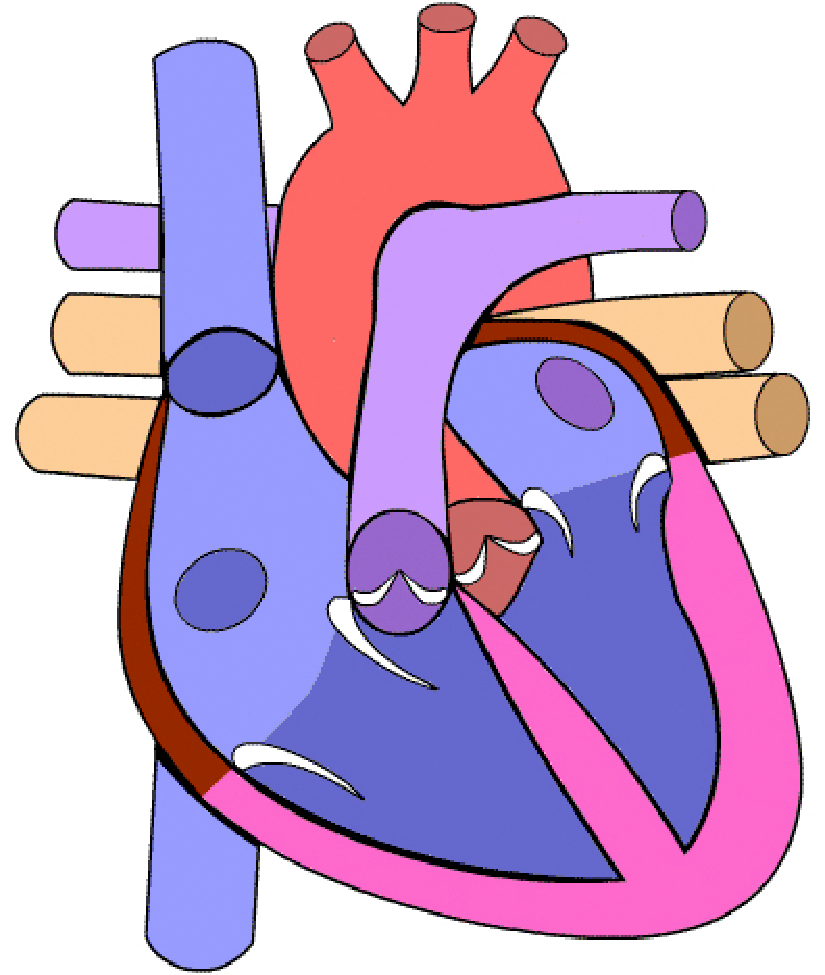
\includegraphics[height=4cm,keepaspectratio]{figure_17}
		\caption[Heart's chambers movement during Atrial systole]{Ventricular pressure continues almost in zero (red line). The arterial pressure continues to decrease slowly (black line), there is a rise in the atrial pressure (dark blue). The ventricles are completely full (light blue) to end-diastolic volume (\SI{130}{\milli\litre}).}
		\label{fig:heart atrial systole}
\end{figure}

%\begin{figure}[!htpb]
%	\centering
%	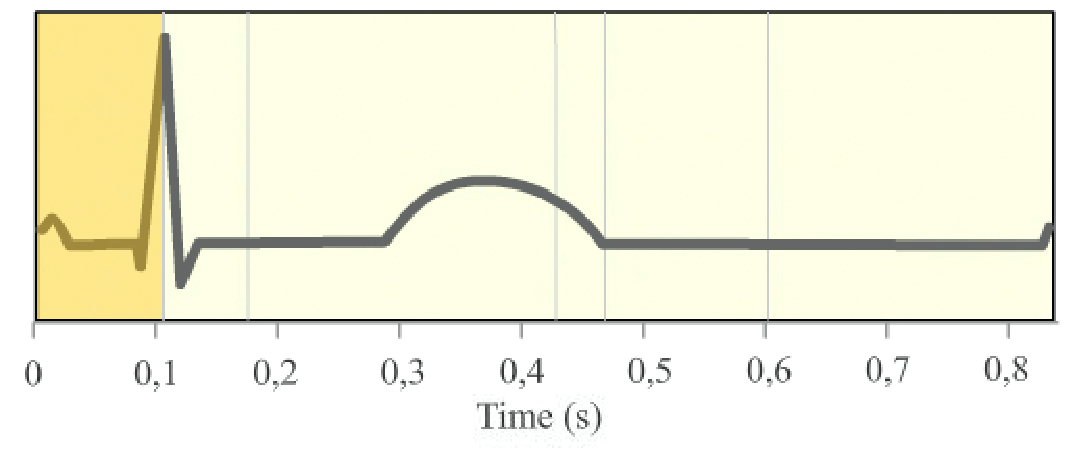
\includegraphics[width=0.5\textwidth,keepaspectratio]{figure_19} 
%	\caption[ECG during rapid ventricular filling]{During rapid ventricular filling there is not electrical activity.}
%	\label{fig:ECG atrial systole}
%\end{figure}
 
\section{Upper limb anatomy}
\label{section literature anatomy}
The experimental work of this document described in chapter \ref{chapter procedure} was carried out in the forearm. This section describes the anatomy of the upper arm and the forearm. This information helps to convey the position of the electrodes and the nearby tissue that interacts with the impedance plethysmography device. 

The arm is part of the upper limb of the human anatomy. It divides into three sections, the upper arm, the forearm and the hand. The upper arm and forearm will be what is explored in more depth as this is what was involved in the study. The upper arm is the section between the shoulder and the elbow and the forearm comprises of the elbow to the wrist. 


\subsection{Bones of the arm}
Figure \ref{fig:upper limb bones} shows the bones of the upper arm of which the humerus being the only bone in this part of the arm. This bone connects the scapula to the radius and ulna which are the bones of the forearm. These bones connect to the carpus bones in the hand which comprises the wrist. The rest of the hand's bones are the metacarpus and the phalanges. 

\begin{figure}[!htpb]
	\centering
	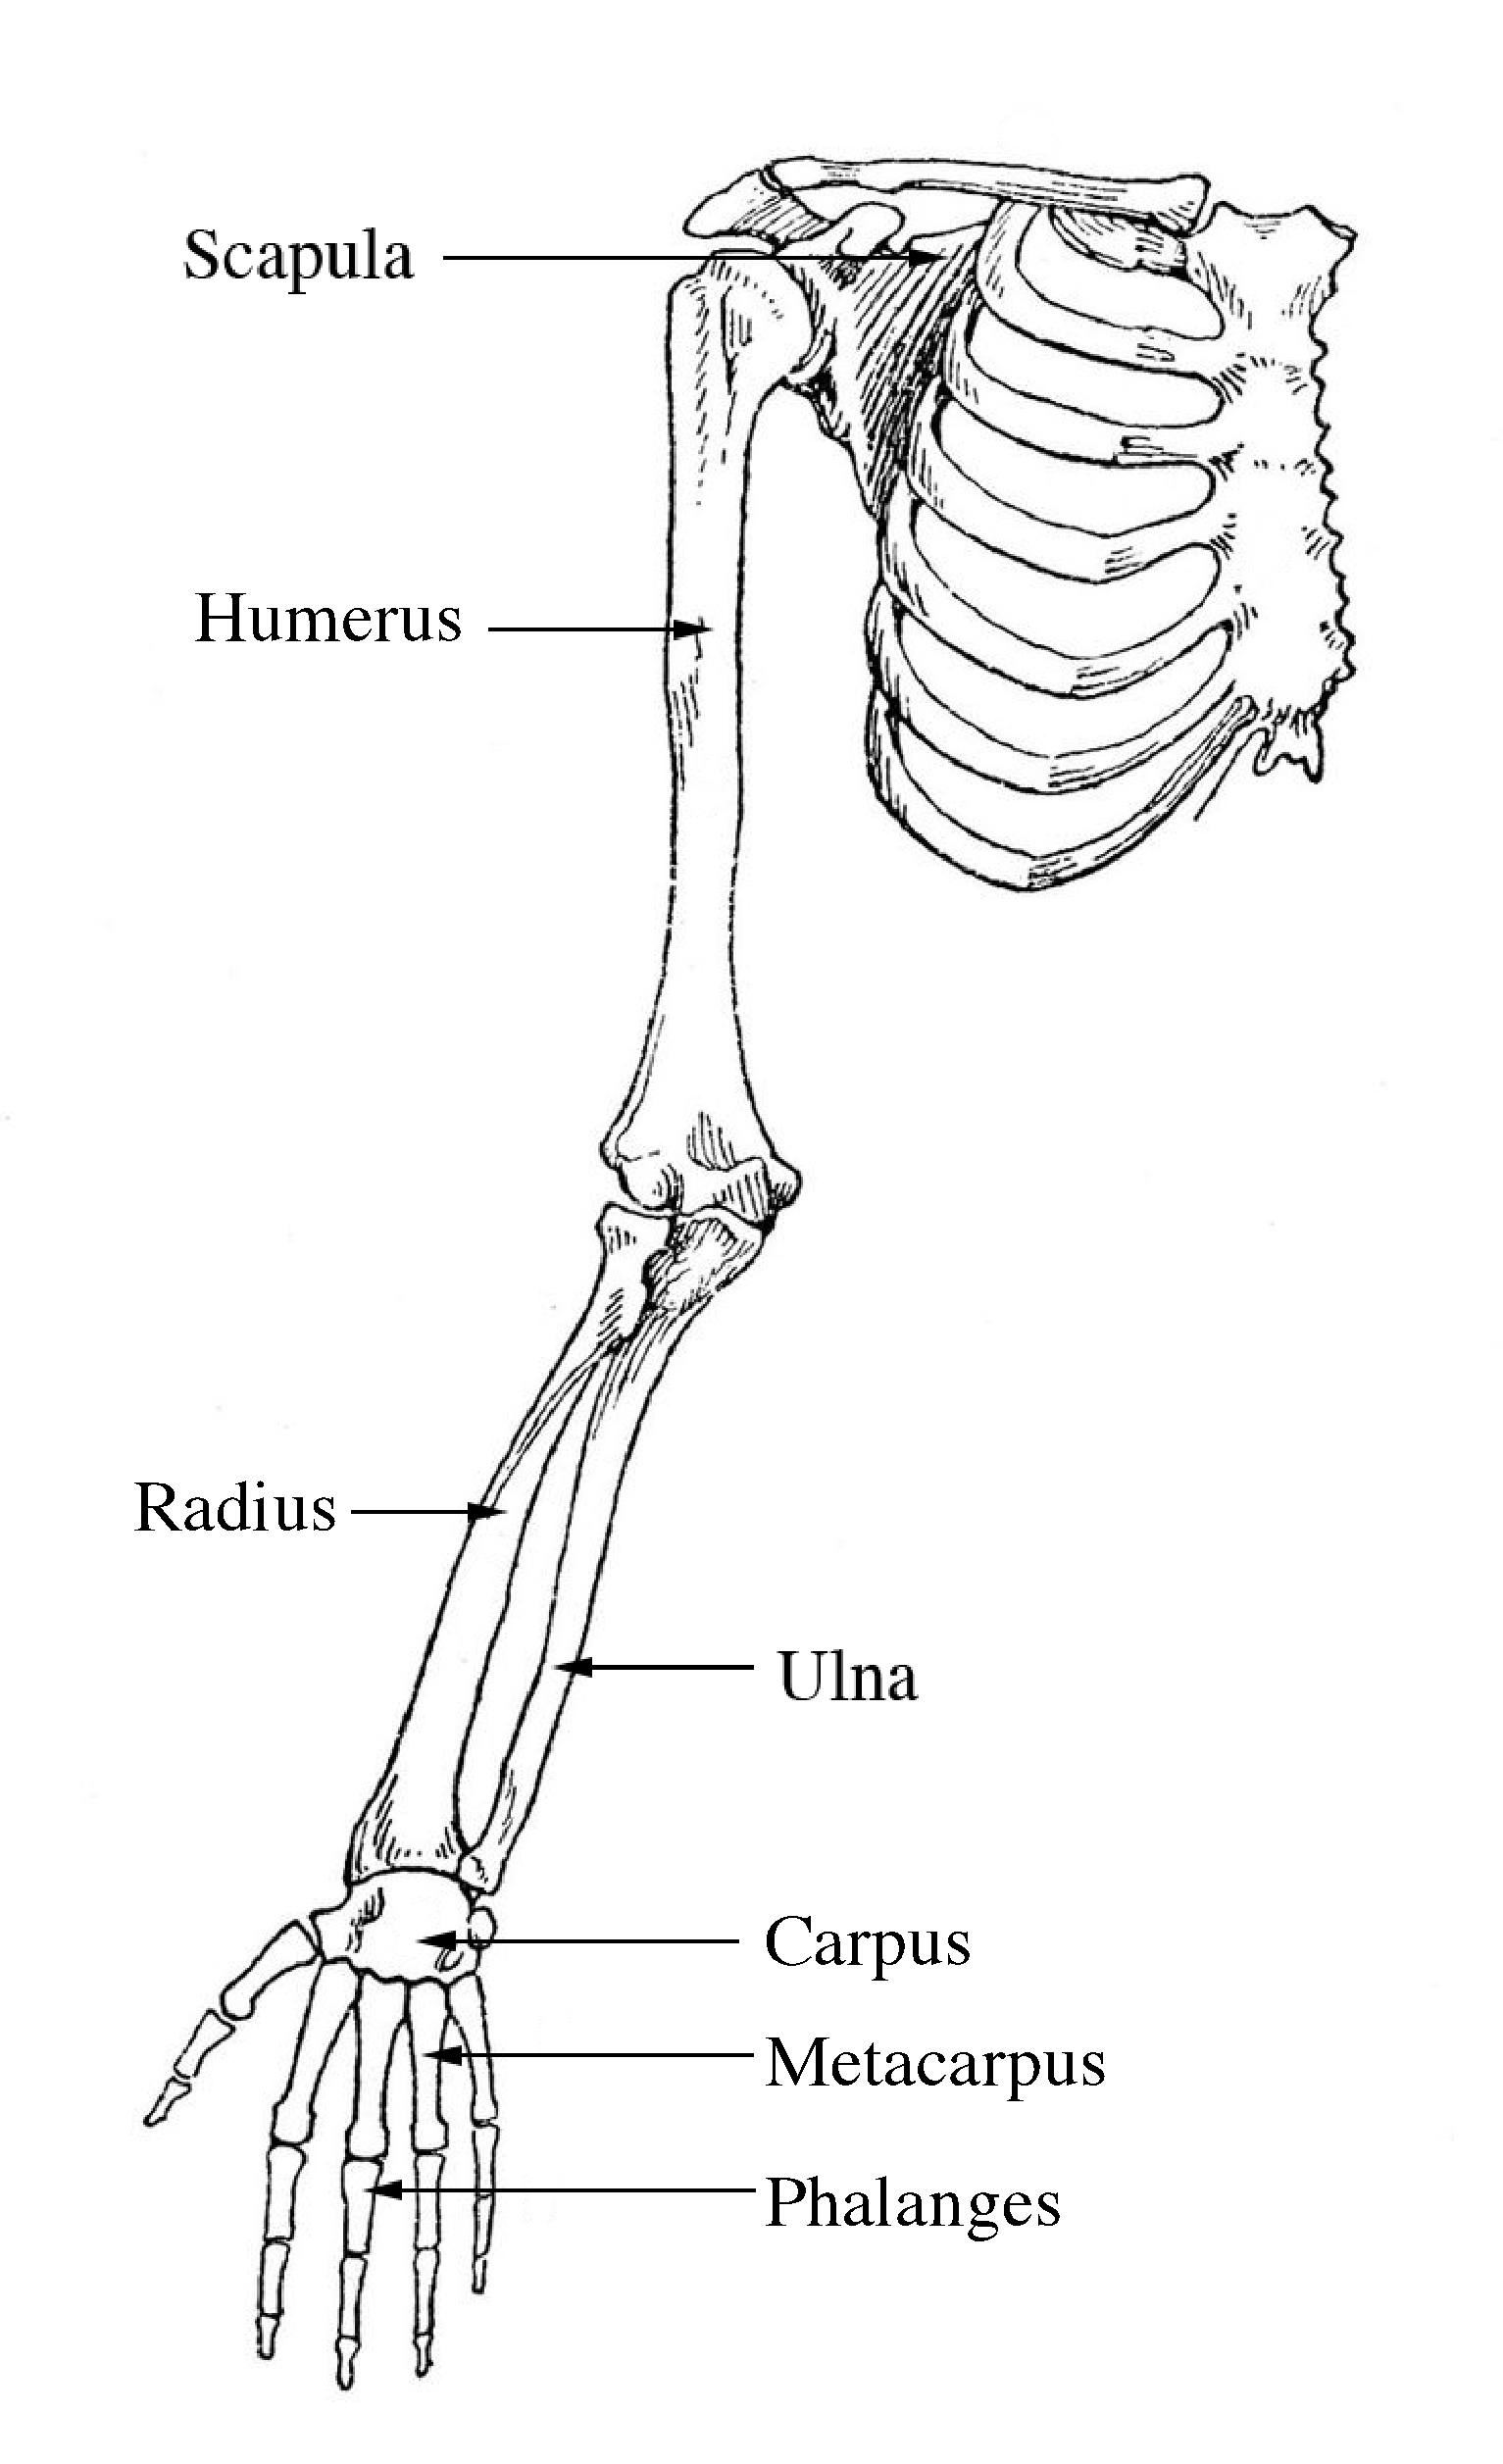
\includegraphics[width=0.4\textwidth,keepaspectratio]{figure_20} 
	\caption{Bones of the upper arm}
	\label{fig:upper limb bones}
\end{figure}


\subsection{Muscles of the arm}
The muscles of the arm are divided by fascial compartments called the lateral and intermuscular septa. This subsequently divides these muscles into the anterior (see figure \ref{fig:upper arm anterior}) and posterior compartments (see figure \ref{fig:upper arm posterior}). The upper arm contains four muscles. Within the anterior compartment are the biceps brachii, brachialis and coracobrachialis, and in the posterior compartment is the triceps brachii. 

\begin{figure}[!htpb]
	\begin{subfigure}[t]{0.52\textwidth}
		\centering
		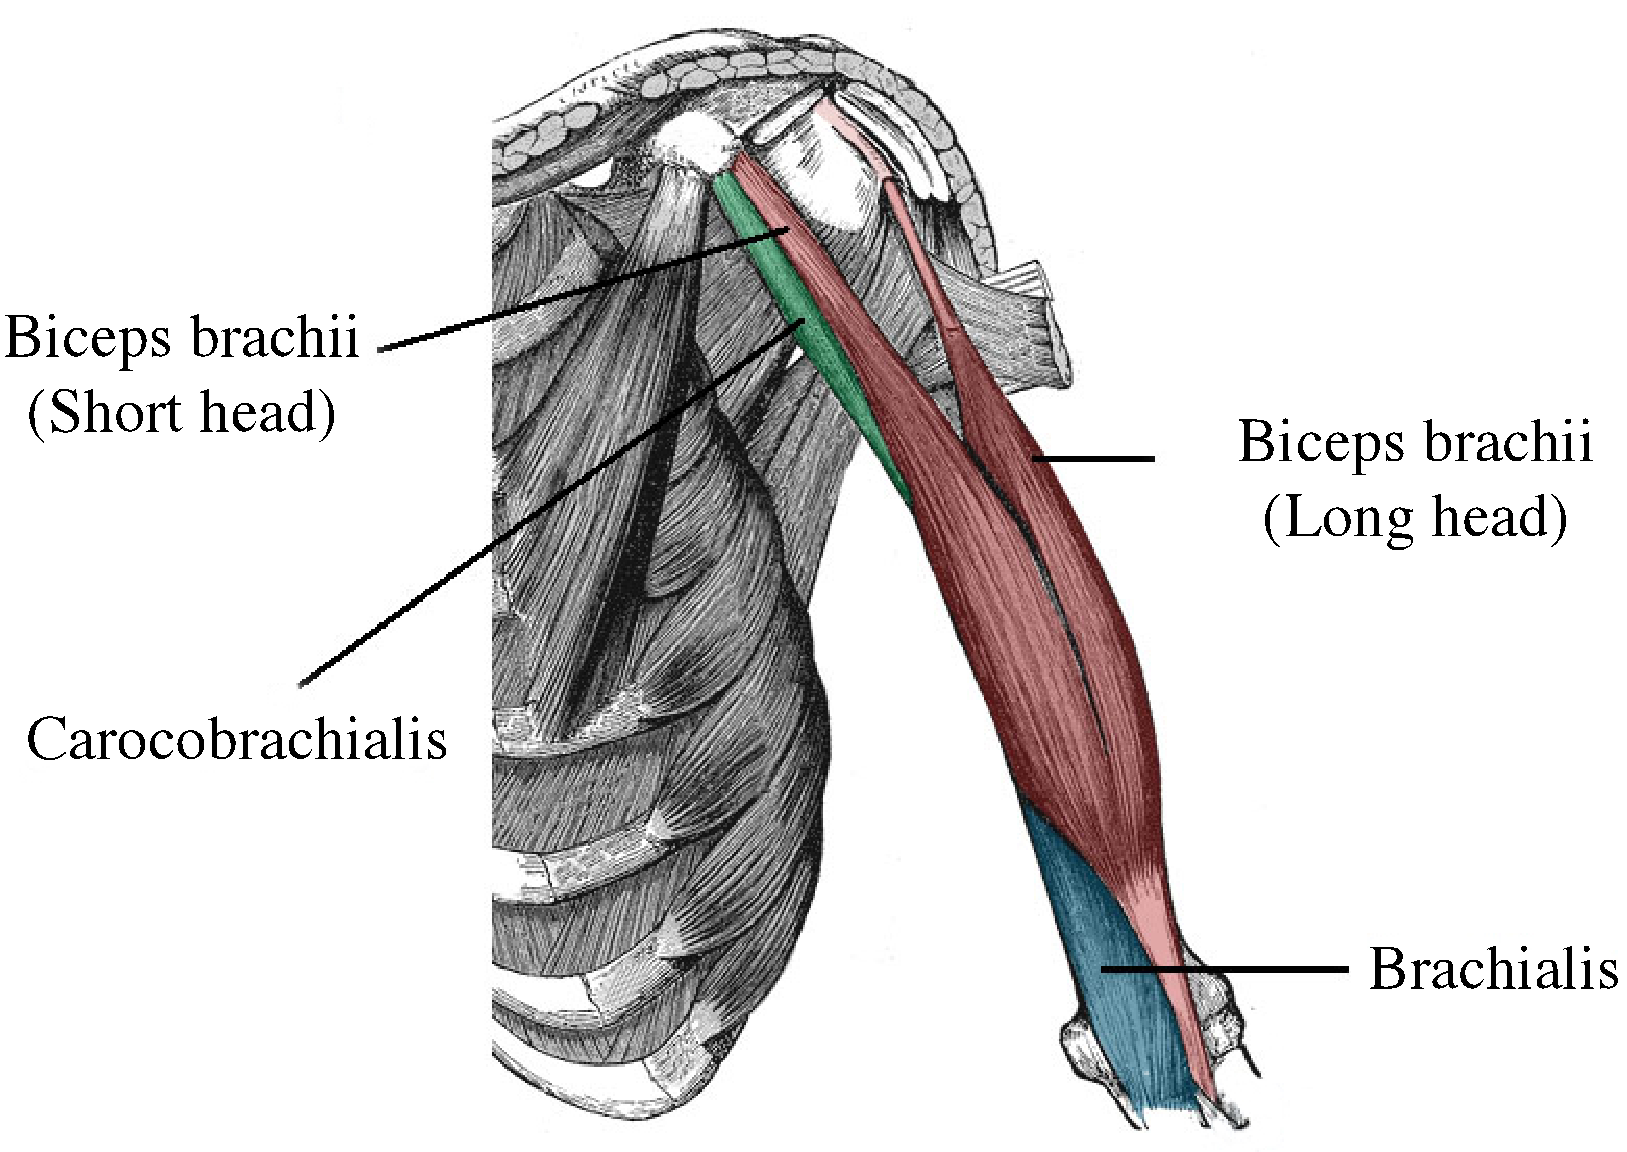
\includegraphics[height=5.5cm,keepaspectratio]{figure15a}
		\caption{Muscles of the anterior compartment}
		\label{fig:upper arm anterior}
	\end{subfigure}
	~
	\begin{subfigure}[t]{0.44\textwidth}
		\centering
		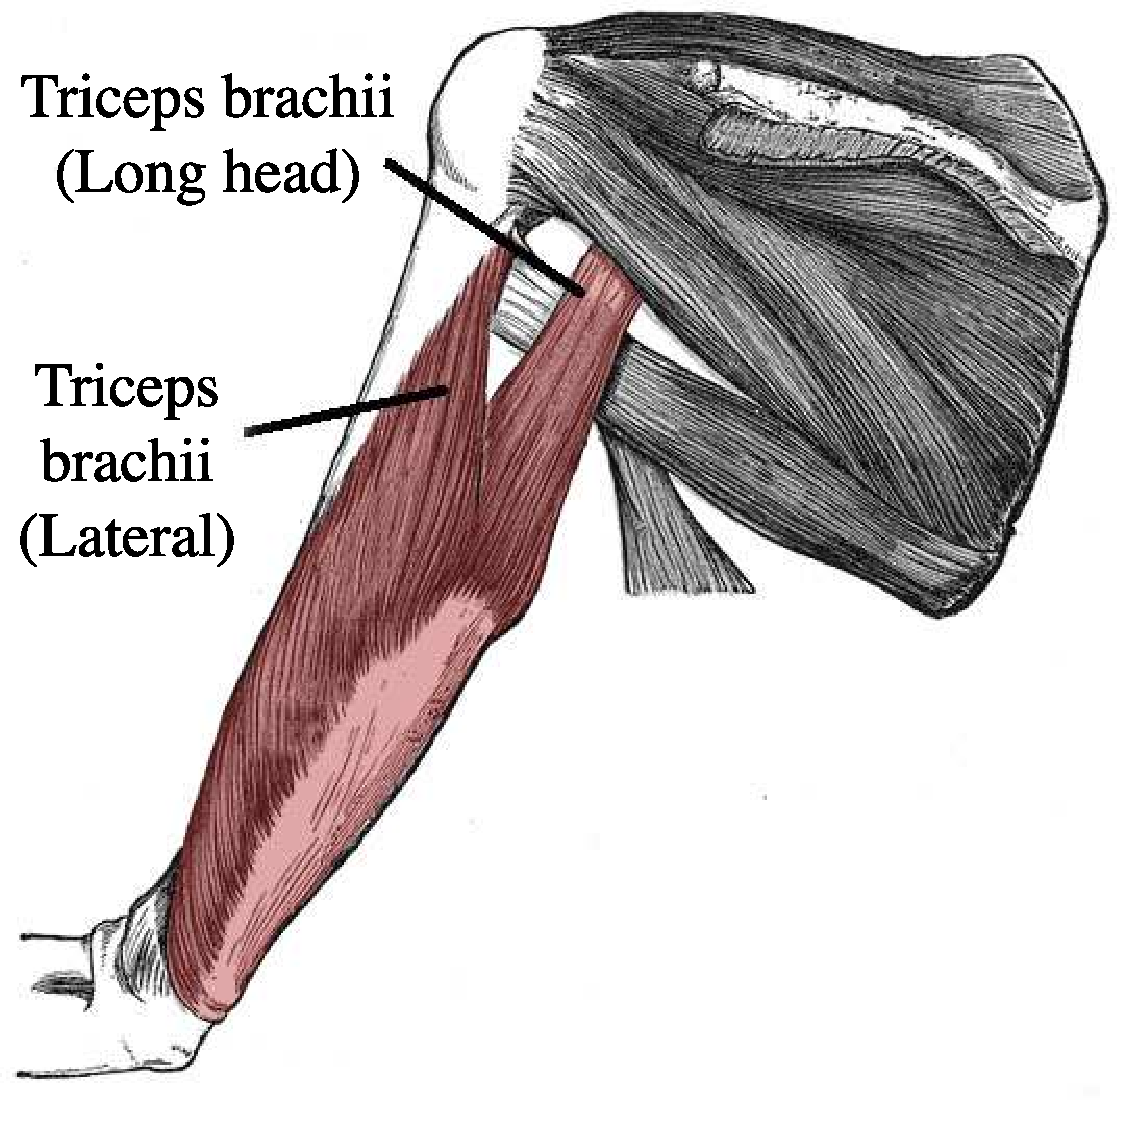
\includegraphics[height=5.5cm,keepaspectratio]{figure15b}
		\caption{Muscles of the posterior compartment}
		\label{fig:upper arm posterior}
	\end{subfigure}
	\caption{Muscles of the upper arm}
\end{figure}

The forearm is composed of many muscles that perform flexion of the wrist and fingers, as well as pronation. The anterior compartment is divided into three; superficial, intermediate and deep. Within the superficial compartment are the flexor carpi ulnaris, palmaris longus, flexor carpi radialis and the pronator teres. The only muscle of the intermediate compartment is the flexor digitorum superficialis. All these muscles are shown in figure \ref{fig:forearm anterior},

\begin{figure}[!htpb]
	\centering
	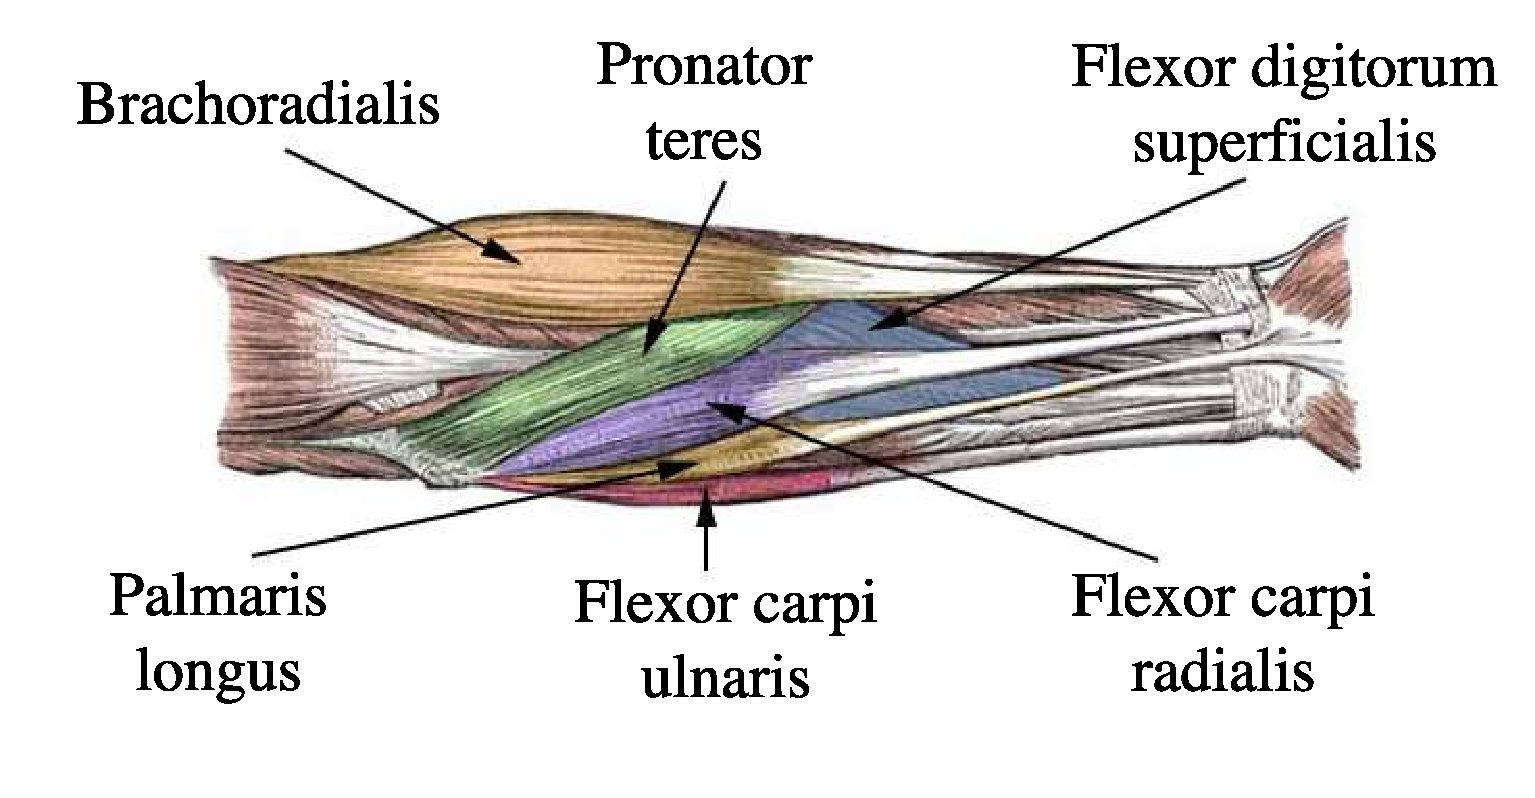
\includegraphics[height=4.5cm,keepaspectratio]{figure16}
	\caption{Muscles of the anterior compartment}
	\label{fig:forearm anterior}
\end{figure}	

Finally, as shown by figure \ref{fig:forearm deep} in the deep compartment three muscles are located; the flexor digitorum profundus, flexor pollicis longus and the pronator quadratus.

\begin{figure}[!htpb]
	\centering
	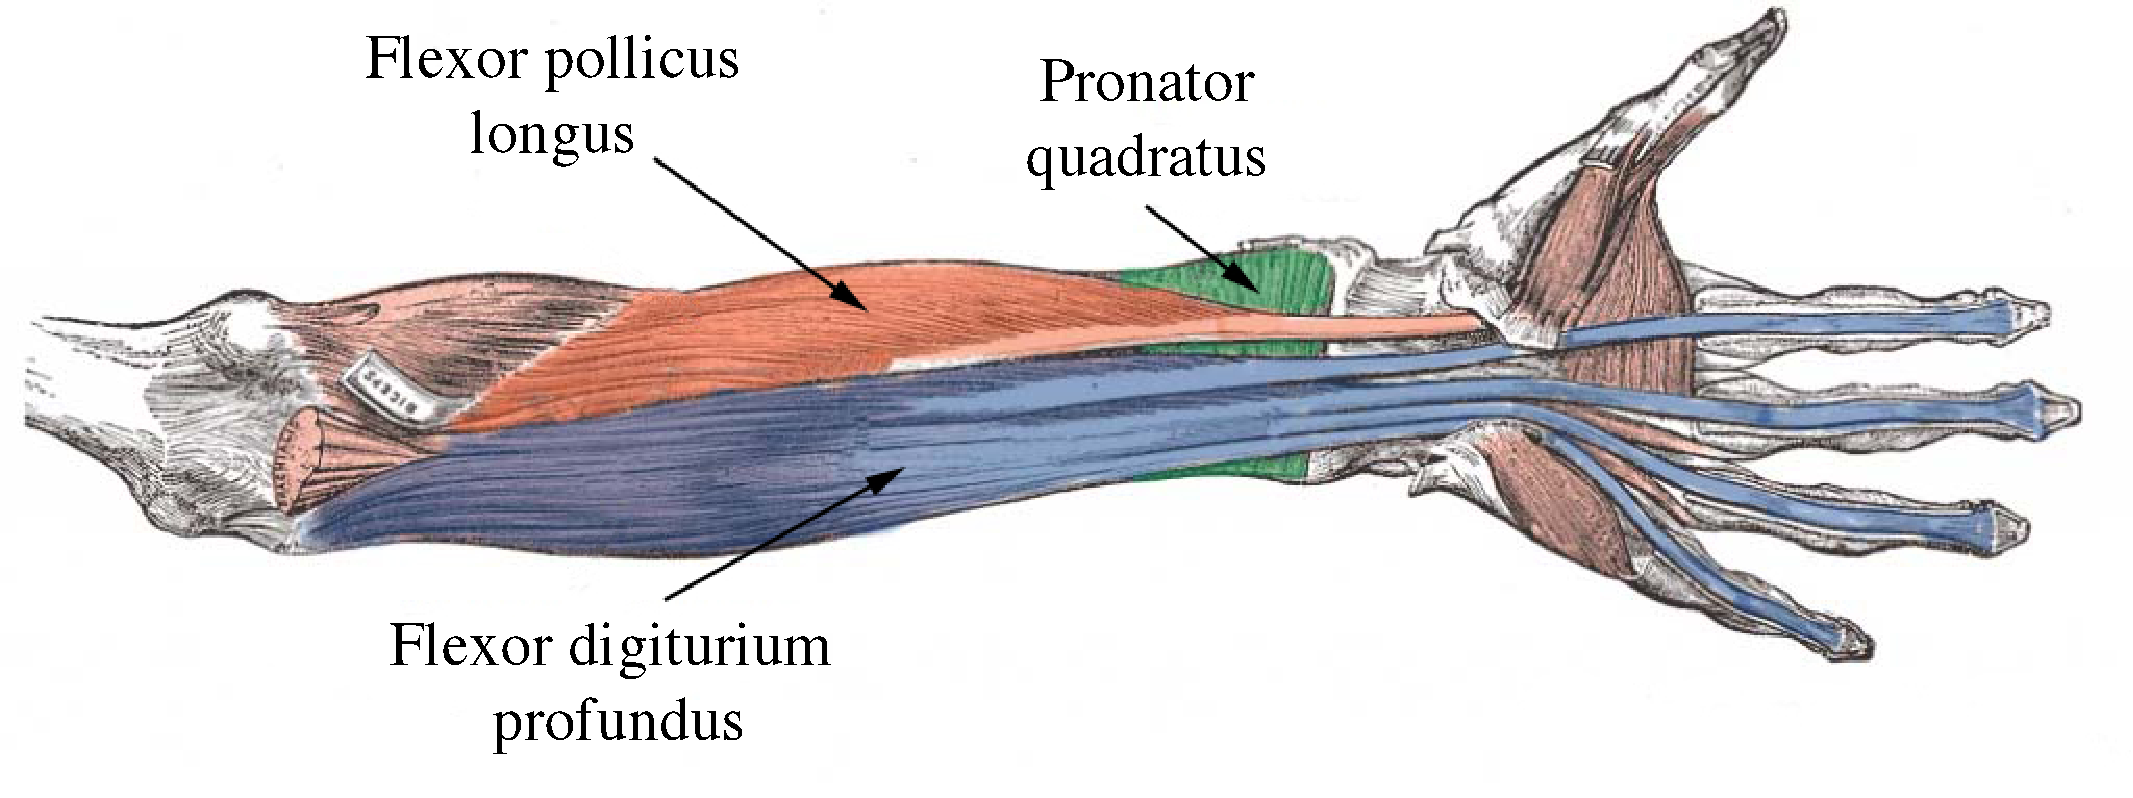
\includegraphics[height=4.5cm,keepaspectratio]{figure17}
	\caption{Muscles of the deep compartment}
	\label{fig:forearm deep}
\end{figure}

\subsection{Circulation of the arm}
\subsubsection{Arterial circulation}
The subclavian arteries located in the chest area supply the blood of the arm.  The right arm blood supply comes from the right subclavian artery which is attached to the brachiocephalic trunk (see figure \ref{fig:subcalvian}). In contrast, the blood supply of the left arm comes directly from the subclavian artery connected to the arch of the aorta. 

\begin{figure}[!htpb]
	\centering
	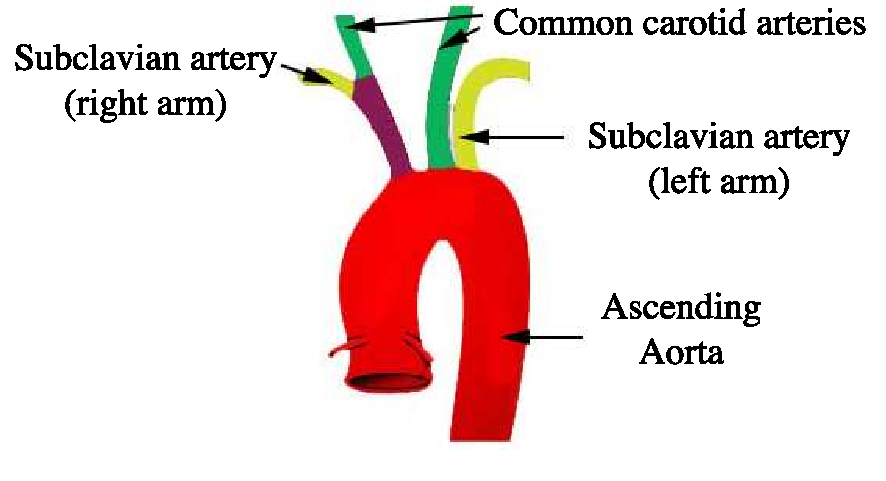
\includegraphics[height=4.5cm,keepaspectratio]{figure18}
	\caption{Origin of the subclavian arteries}
	\label{fig:subcalvian}
\end{figure}

When these arteries pass through the axilla, they are known as axillary arteries. From this artery, other arteries arise such as the posterior and anterior circumflex arteries which supply blood to the shoulder section, and the subscapular artery which is the largest. 

Hereafter, as shown in figure \ref{fig:upper arm circulation} the axillary artery becomes the brachial artery at the teres major muscle, which is the blood supply for the whole arm.  From this artery, other arteries arise that supply blood to the tissues in the upper arm. Such as the profunda brachii which is the deep artery of the arm travelling around the posterior surface of the humerus. 

\begin{figure}[!htpb]
	\centering
	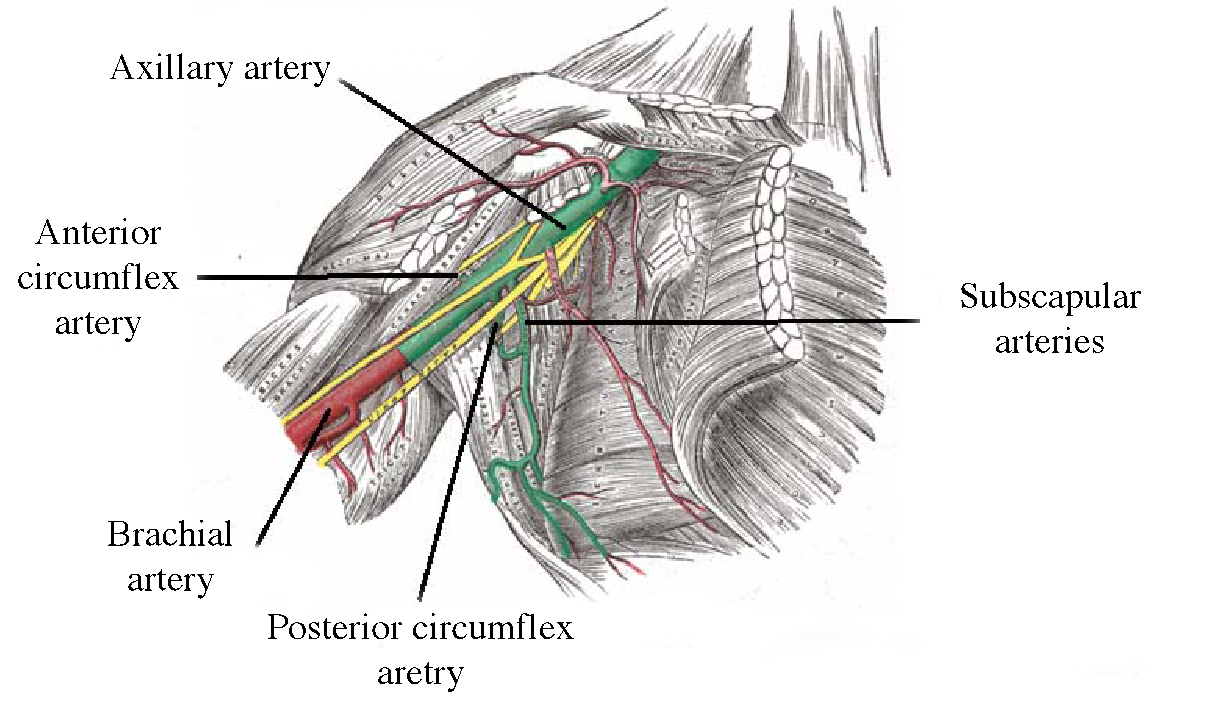
\includegraphics[height=6cm,keepaspectratio]{figure19}
	\caption{Origin of the subclavian arteries}
	\label{fig:upper arm circulation}
\end{figure}

As can be seen in figure \ref{fig:forearm aretries}, as soon as the brachial artery passes the cubital fossa (front of the elbow joint) underneath the brachialis muscle, this artery bifurcates becoming the radial and ulnar arteries. The radial artery supplies blood to the posterior tissues of the arm and the ulnar to the anterior. At the carpus bones, these arteries anastomose in the hand forming the superficial and deep palm arches which provide blood to the different tissues located in the hand. 

\begin{figure}[!htpb]
	\centering
	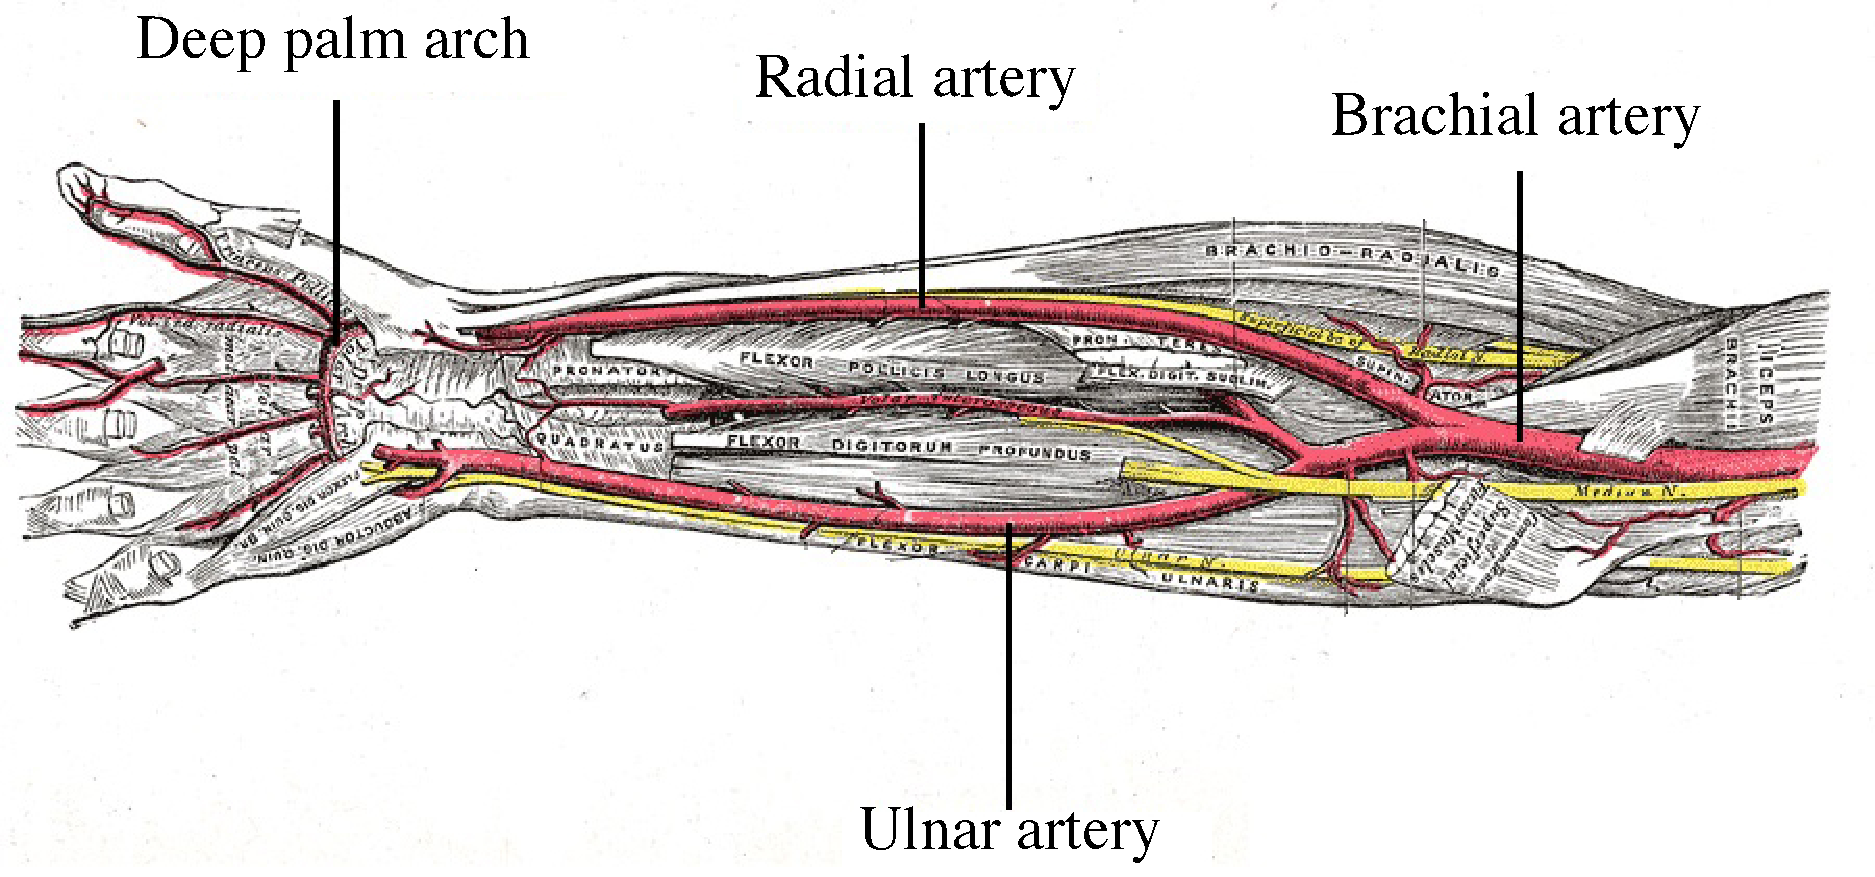
\includegraphics[height=4.5cm,keepaspectratio]{figure20}
	\caption{Forearm arteries}
	\label{fig:forearm aretries}
\end{figure}

\subsubsection{Venous circulation}
The veins of the arm are anatomically split into the superficial and the deep veins (see figure \ref{fig:arm veind}). The largest superficial veins in the upper limb are the cephalic and basilic veins. The latter originates at the venous branches of the hand, near the teres major at which point the vein goes deep into the arm. At this point, this vein combines with the brachial veins to form the auxiliary vein. 

The cephalic vein begins at the dorsal venous network of the hand. It ascends on the anterolateral region of the arm and at the elbow passes to the anterior part of the limb. In this same section, the median cubital vein connects the cephalic and basilic veins. At the axilla, the cephalic vein joins to the axillary vein. 

The deep fascia contains the deep veins in the upper limb. These veins are paired to either side of the brachial, radial and venous artery. Hence, they inherited the same names.  In fact, the pulsation of the brachial artery helps the venous return of the arm. This effect is known as vena comitantes. The perforating veins connect the deep and superficial veins of the upper arm. 

\begin{figure}[!htpb]
	\centering
	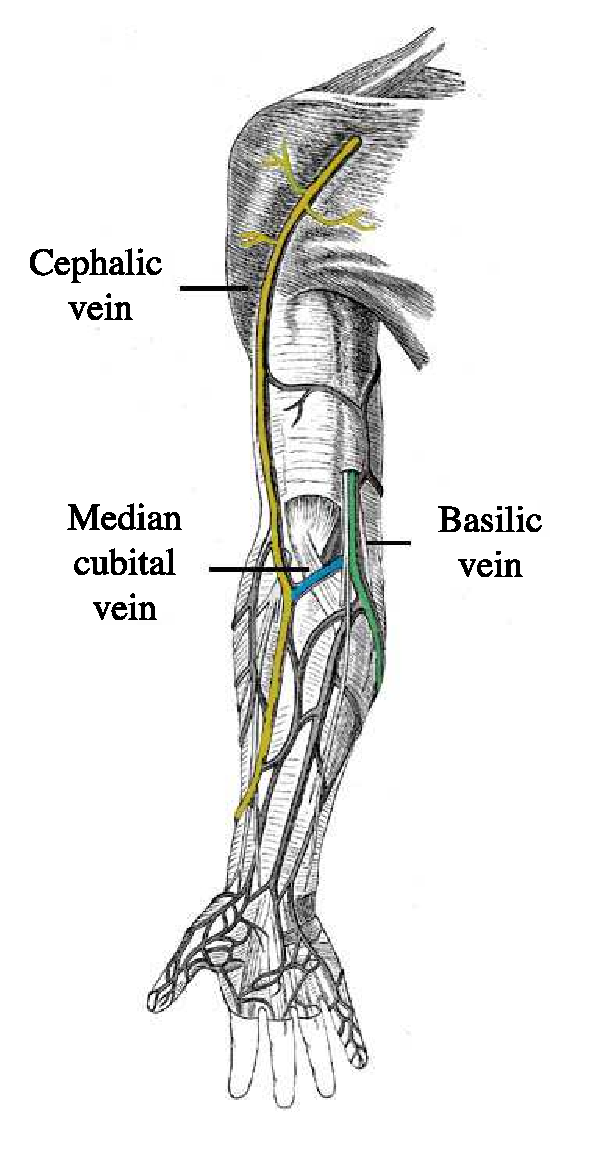
\includegraphics[height=10cm,keepaspectratio]{figure21}
	\caption{Forearm arteries}
	\label{fig:arm veind}
\end{figure} 

%********************************** %Section 2.1.2  **************************************
\section{Oxygen transportation}
\label{section literature 1.2}
Oxygen ($O_2$) is an essential component needed by all of the body's cells to complete metabolic processes. Within the blood, this is transported by haemoglobin (Hb) contained inside red blood cells (RBCs). Oxygen is required for the chemical reactions needed to convert biochemical energy from nutrients coming from food into cell's energy known as coenzyme or adenosine triphosphate (ATP). As a result of this reaction a waste product is released from the cell. A human cell can only survive for a few minutes without oxygen~\cite{culmsee2005apoptosis}.

Inadequate oxygen delivery to the body's tissue is known as hypoxia. There are different classifications of hypoxia  based on its cause~\cite{marieb2007human} which are described as follows: 

\begin{enumerate}
    \item \textbf{Anaemic Hypoxia:} It is a condition where a body part or an organ has poor $O_2$ delivery. Some of the causes are a small count of RBCs and abnormal or too little Hb content in the blood's cells.
    \item \textbf{Ischaemic (stagnant) hypoxia: }This is caused when blood circulation is reduced or blocked. There are different causes for this. However, the most common are congestive heart failure that may cause body–wide hypoxia, emboli or thrombi blocking oxygen supply to the tissue distal from the occlusion. 
    \item \textbf{Histotoxic hypoxia: }Mainly caused by metabolic poisoning like ingestion of cyanide. In this case the cell is unable to use $O_2$ for metabolic purposes, even though there is an appropriate amount of $O_2$ being delivered by the body.
    \item \textbf{Hypoxemic hypoxia:} It is shown by a decrease in the arterial oxygen partial pressure ($PO_2$). Some of the causes are an imbalance in the ventilation–perfusion coupling mechanism, poor ventilation caused by pulmonary disease and breathing air with a low content of $O_2$. Moreover, carbon monoxide ($CO$) poisoning is another reason behind this illness because it has \num{200} times more affinity with Hb than $O_2$. Thus, in places with high concentrations of CO such as with fires, this could easily lead to death.
\end{enumerate}




%********************************** %Section 2.2  **************************************
\subsection{Problems derived from poor blood delivery} %Section 4,1
\label{section literature 4,1}
Now that some of the problems of having poor oxygen transportation at a cellular level have been touched on, more detail will be unveiled about illnesses due to the poor or total lack of blood delivery to human tissue, especially human limbs. 

Ischaemia develops when there is an insufficient supply of blood to an organ. For instance, if an artery blockage occurs, all the tissue below the blocked path will suffer from starvation of oxygen and other critical nutrients. Different causes could lead to the blockage of an artery these can be by external or internal factors. Speaking specifically about lower limbs, ischaemia represents a significant cause of disability and cardiovascular morbidity and mortality~\cite{novo1995patients}.

Different kinds of diseases exist compromising limbs, an example of this is peripheral arterial disease (PAD), of which there are two subtypes. One of these is critical limb ischaemia (CLI), whereby if a medical intervention is not given quickly enough the patient could loose their limb. One of the first symptoms of this condition is that the patient experiences continuous pain in the extremity even at rest ~\cite{novo2004critical}. 

Clinically there are different methods to assess the development of this illness. Some scales of qualitative evaluation have been developed such as the Rutherford classification, the Leriche-Fontaine classification or the TACS II classification of femoral and popliteal lesions~\cite{norgren2007inter}. Health practitioners use a survey, an indicator of pain when walking and a visual inspection. With this it is possible to determine the stage or the severity of the arterial occlusion.  Table \ref{table:Fontaine}) shows the different stages of the Leriche-Fountain classification and the various steps considered to evaluate the illness.

\begin{table}
\caption{Leriche-Fontaine classification}
\centering
\label{table:Fontaine}
\begin{tabular}{p{1.8cm} >{\raggedright}p{3.6cm} p{3.4cm} p{4.8cm}}
\toprule
\textbf{Stages}& \textbf{Symptoms} & \textbf{Pathophysiology} & \textbf{Pathophysiological \newline classification} \\
\midrule
Stage I & Asymptomatic or effort pain & Relative hypoxia & Silent Arteriopathy \\
\midrule
Stage II A & Effort pain \newline Pain free walking distance > \SI{200}{\meter} & Relative hypoxia & Stabilized Arteriopathy \newline Non-Invalidant claudication \\ 
\midrule
Stage III A & Rest Pain \newline Ankle arterial pressure > \SI{50}{\mmHg} & Cutaneous hypoxia \newline Tissue acidosis \newline Ischemic neuritis & Instable arteriopathy \newline Invalidant claudication \\
\midrule
Stage III B & Rest pain \newline Ankle arterial pressure < \SI{50}{\mmHg} & Cutaneous hypoxia \newline Tissue acidosis \newline Ischemic neuritis & Instable arteriopathy \newline
Invalidant claudication \\
\midrule
Stage IV & Trophic lesions \newline Necrosis or Gangrene & Cutaneous hypoxia \newline 
Tissue acidosis & Necrosis \newline Evolutive arteriopathy \\
\bottomrule
\end{tabular}
\end{table}

As table~\ref{table:Fontaine} shows, there are various levels of stratifying the severity of the disease according to symptoms which are related to pathophysiology. There are also different methods to examine the severity of the disease using imaging techniques.

There are a significant number of illnesses that are derived from the inadequate delivery of blood towards a limb. According to their physiology, they can be divided into a disease which affects either the microcirculation or main vessels or both. The following are just an example of the different diseases that may require continuous blood flow monitoring in acute or chronic settings.



%********************************** %Section 2.2.1  **************************************
\subsubsection{Peripheral vascular disease}
\label{section literature 2.1}
The name of the disease which causes the reduction of blood towards a limb is known as peripheral vascular disease (PVD) and also sometimes called peripheral arterial disease (PAD). This illness is a progressive vascular condition caused by the blockage, narrowing, or spasms in a blood vessel (arteries, veins or lymphatic vessels). Thereby, altering the blood circulation to and from upper or lower extremities.  It most commonly affects the lower limbs, particularly most distally. Therefore, the derivation of its name as \textit{peripheral} because it affects mostly the periphery of the body. It affects \SI{5}{\percent} of people over \num{50} and between \SIrange{12}{20}{\percent} of people over 65 years old. To some extent, it is more common in men than women. People with certain risk factors are more likely to suffer PVD such as patients with diabetes or smokers as some studies have demonstrated \cite{kannel1979diabetes,janka1980peripheral, menzoian1989symptomatology, eliasson2003cigarette, stephens2004cardiovascular}. It is more likely that patients with diabetes may develop occlusion of large arteries in the lower extremities that also could lead to gangrene and ulcers. In contrast, smokers may present intermittent claudication, in other words, pain, cramp, numbness or sense of muscle fatigue. 

Different factors could cause the narrowing of the blood vessels. The most common cause of PVD is atherosclerosis, the deposit of fatty material on the arterial walls. This fatty material constitutes a plaque that reduces the blood flow. This in turn, lessens the transport of $O_2$ and nutrients as explained previously in section \ref{section literature 4,1}. Moreover, this uneven deposit increases the chances of clots to form on the artery walls reducing the internal size of the vessel and increasing the risk of obstructing a major artery.

Different risk factors are contributing to the development of this illness. Some can be inherited, others are based on lifestyle choices. The combination of two or more of the following risks may increase complications from PVD, such as smoking and diabetes.To expand on this in more detail, some of the documented risk factors are: \rvmynote{This needs to be referenced}

\begin{itemize}[noitemsep]
    \item Age (especially over \num{50})
    \item Family history (high blood pressure, high cholesterol or PVD)
    \item Diabetes
    \item Smoking
    \item Obesity
    \item Infections
    \item Coronary artery disease
    \item Injury to vessels
    \item Physical inactivity
    \item High blood pressure
    \item Autoimmune diseases
    \item Nutritional deficiencies
    \item High blood cholesterol
    \item Emboli from other locations in the body
    \item Inflammation of the blood vessels
\end{itemize}

In the first stages of the illness, symptoms are not noticeable, which makes the condition difficult to diagnose. The most common presentation is when it has progressed to the extent of causing pain as described by the Fontaine's classification (see table \ref{table:Fontaine}). However, performing a qualitative assessment of the extremity helps to diagnose the illness at earlier stages. This assessment uses indicators such as coldness of the extremity to touch, poor skin condition (thinning, shining or brittle), poor nail health (thickening or opaque nails), hair loss in the extremity, reduced pulse sensation in the extremity, impotence, infections or injuries not healing properly, poor muscle condition (numbness, weakness or heaviness), pain while walking and stopping at rest, local skin discolouration (pale, blue or dark red) and restricted mobility \cite{morgan2001developing, norgren2007inter}.

Once a qualitative or physical examination has been performed, and the progress of the illness has been classified, there are additional tests that may help to diagnose the severity of the PVD. Some of the methods just require the assessment of the medical practitioner using common medical devices, others may need the use of specialised equipment. Some of the therapeutic methods that do not demand the use of bulky or cumbersome devices are:

\begin{itemize}
    \item \textbf{Ankle-brachial index (ABI):} This is the ratio of the differential measurement of systolic blood pressure measured at the ankle to that measured at the brachial artery \cite{winsor1950influence}. This means one must compare the difference in blood pressure between the arm and the ankle, as well as recording the ankle's blood flow using a Doppler ultrasound instrument.  
    \item \textbf{Treadmill exercise test: }In this method the patient has to walk or run to monitor the circulation during exercise. Pain or problems during the test are recorded to examine the severity of the obstruction.
    \item \textbf{Reactive hyperaemia test:} This test refers to a temporary increase (\textit{hyper}) of blood flow (\textit{emia}) of the extremity. It is usually performed in people who are not able to walk on a treadmill. In this case, the person remain in supine position, and comparative measurements of blood flow are taken using a Doppler Ultrasound instrument in the thighs and ankles. Then, after an occlusion is applied in the limb comparing any decrease in the flow rate between both sites. 
\end{itemize}

%********************************** %Section 2.2.2  **************************************
\subsubsection{Compartment syndrome}
\label{section literature 2.2}                                                                                                                                                                                                                                                                                                                                                                                                                                                                                                                                                                                                                     
All the muscles, blood vessels and nerves are contained within a tissue known as fascia. When the pressure in a limb within this compartments increases because of bleeding or swelling, it could lead to total or partial restriction of micro–vascular blood flow \cite{songer2001tissue}. Some cases may present with rapid discolouration and blistering of the affected limb which is commonly associated with oedema, cyanosis and severe pain \cite{chhabra2013compartment}. Hence, it can lead ultimately to venous hypertension and loss of blood plasma. If the arterial flow is reduced, it may also result in gangrene, limb loss or even death \cite{lamborn2014compartment}. This syndrome can be catalogued as acute when it is caused by either an injury, accident or medical emergency, and chronic when it occurs gradually during any sports activity.

The most common method to diagnose this illness is Doppler sonography \cite{chhabra2013compartment}. Nevertheless, detecting foot compartment syndrome could be challenging compared to other parts of the body because its symptoms and indicators are less reliable \cite{dodd2013foot}.

%********************************** %Section 2.2.3  **************************************
\subsubsection{Diabetic foot infection}
\label{section literature 2.3} 
The lack of blood towards an extremity can also be caused by a secondary effect of other illnesses such as diabetes. Some of the most common problems that diabetic patients have to deal with are diabetic foot infection which is a clinical syndrome characterised by local findings of inflammation or purulence in a person with diabetes. This disease also leads to a decrease in peripheral circulation, vascular disease and loss of nerve sensation ending up in the formation chronic ischaemic ulcers and bacterial infection. Diabetes is the leading cause of lower extremity amputation in developed countries, and it is responsible for \SI{60}{\percent} of these amputations~\cite{ucckay2014diabetic}.  Currently, Doppler ultrasound flowmetry is still one of the primary tools to diagnose the advance of diabetes foot infection (DFI). New techniques to follow up the progress of this illness have been researched, such as bioelectrical impedance~\cite{cheng2012application}, planar pressure analysis~\cite{dos2010insole}, imagine technique analysis~\cite{songer2001tissue}, near infrared~\cite{papazoglou2008assessment} and electronic noses~\cite{yusuf2013diagnosis}. Until now, nothing has been designed to detect early stages of this problem before ulceration occurs. With regards to bioelectrical impedance analysis (BIA), there have been studies focused on the detection on the development of ischaemia of the foot's sole showing a good correlation with laser Doppler flowmetry~\cite{cheng2012application}. 

% I decided to remove this section as It does not relate completely to flow and focus to instrumetns that measure blood flow in periphery
%\section{Methods to measure volume and flow}
%
%
%\subsection{Instruments to measure volume}
%\label{section literature 3}
%The word plethysmography roots from the Greek word \textit{plethymos} that means either increasing or enlarging and \textit{graphos} that is to write. In other words, it can be defined as the measurement of any volume within the human body. In medicine, some of the common applications are the measurement of volume changes in lungs caused by the respiratory system or blood vessels caused by the circulatory system~\cite{turcott2004methods}. More specifically when referring to the latter, plethysmography aims to measures the pulsatile volume changes when the heart pumps blood in and out of a segment of the human body. 
%
%A plethysmography device produces an output waveform that is synchronous to the heart cycle. The shape of the signal is similar to an arterial pressure waveform. In fact, the plethysmography plot represents the volume of the arterial vasculature obtaining a measure of the arterial pulse amplitude. This waveform gives meaningful information about the pulse velocity and indications of possible arterial obstruction.
%
%\begin{figure}[!htpb]
%	\centering
%	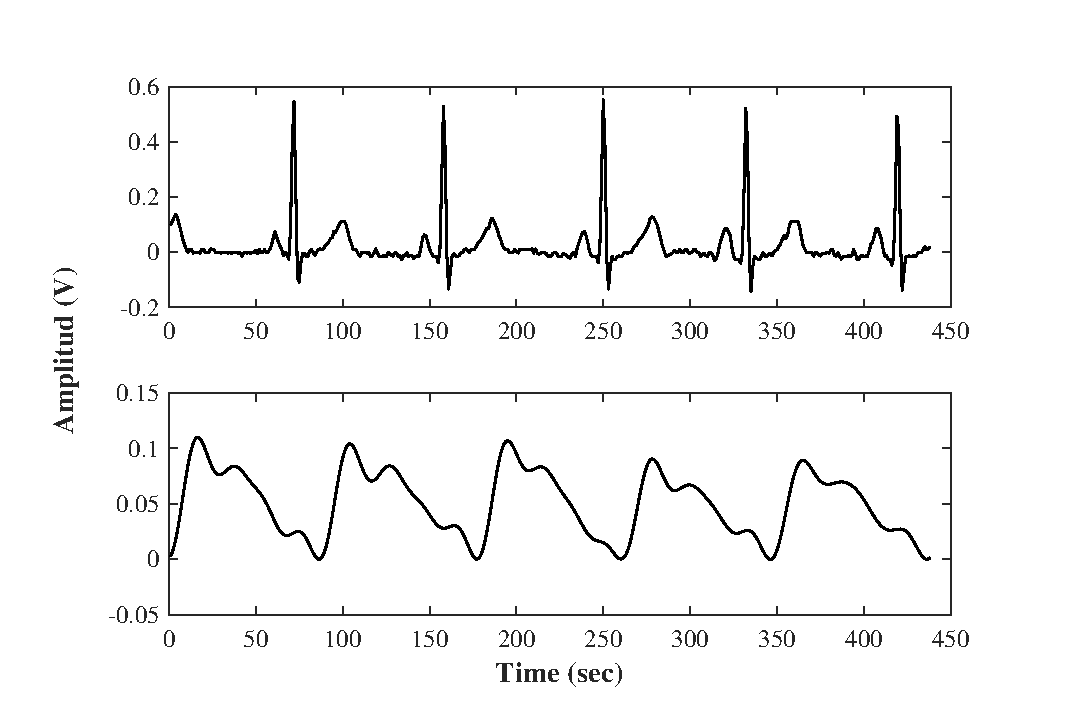
\includegraphics[width=0.75\textwidth,keepaspectratio]{figure3}    
%	\caption[Classic plethysmography waveform]{Representation of a classic plethysmography waveform from the heart cycle. The image on the top represents the electrical signal of the heart (ECG). The one below is the plethysmography waveform of the circulation. Both signals are synchronous}
%	\label{fig:plethysmography}
%\end{figure}
%
%There are different methods and technologies to measure plethysmography. Every method can be applied separately or as part of a system. Some techniques can measure plethysmography of the whole body, segments or localised areas. For instance, chambers of air or water are used to measure lung capacity. It works by placing the patient in the chamber and measuring the total volume during inhalation and exhalation. Thus, the lung capacity can be calculated as the total displacement of air or water during a respiratory cycle. 
%
%For measurement of changes of volume of a limb's segment, the air plethysmography technique could be very cumbersome and not very practical for an ambulatory or home setting. For instance, measuring plethysmography with this method requires a whole chamber that immobilise completely the arm. Therefore, it is not pratical for self-measurements. The following section explain more in detail the pros and cons of the methods used to measure the change of volume in the body.
%
%\subsubsection{Air plethysmography}
%\label{section literature 3.1}
%Air plethysmography is not a common method to measure a limb’s change of volume. It has been used as an alternative or research method as explained by Chuah et al.~\cite{chuah2004plethysmography} for measurement of plethysmography without venous occlusion. This approach uses a special chamber that contains the limb in a closed area with orifices where transducers and calibration devices are connected. The arm is introduced into the case through a tight rubber sleeve to ensure that the instrument is airtight.  The plethysmography pulsations are detected by measuring the displacement of the surrounding air with a sensor connected to the chamber, which also moves the rubber diaphragm whereby a Doppler ultrasound transducer measures displacement. 
%
%This method can provide quite accurate results but motion artefact causes ripples movements that affect the final value. Furthermore, this method could be burdensome for a home setting or even for surgery applications. It requires and extra participant to aid positioning the arm within the chamber and perform the adequate calibration.
%
%\begin{figure}[!htpb]
%	\centering
%	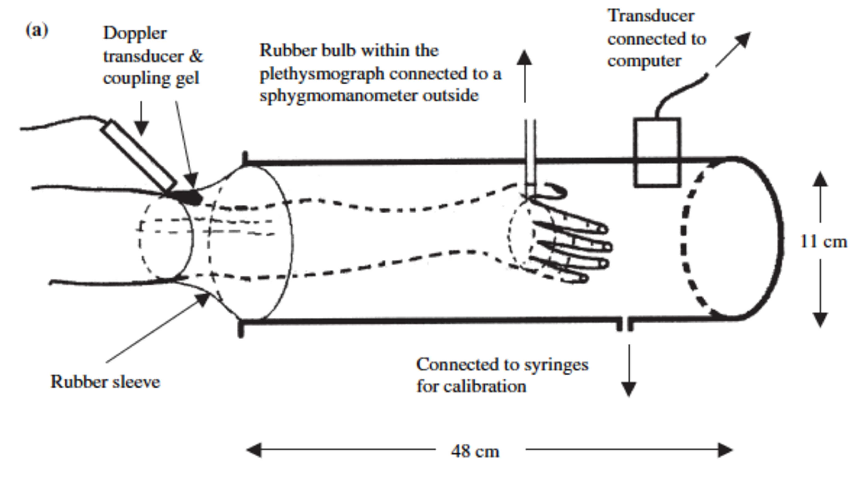
\includegraphics[width=0.95\textwidth,keepaspectratio]{figure4}    
%	\caption[Air plethysmography method]{Representation of an air plethysmography device. It requires a one side open cylinder with a rubber sleeve. There is a compartment where the air displacement caused by each cardiac cycle can be measured.}
%	\label{fig:air plethysmography}
%\end{figure}
%
%\subsubsection{Strain gauge plethysmography}
%\label{section literature 3.3}
%This method also known as SGP (strain gauge plethysmography) is a non-invasive method to quantify retrograde outflow in the deep venous system and peripheral arterial disease~\cite{holohan1996plethysmography}. It works by applying a strain gauge around the limb under test\mynotenp{under test??}. The transducer could be a tube filled in with a conductive material such as mercury and gallium and connected to a source of electricity. However, alternative methods that do not use clinically banned mercury have been developed using electrical conductive fluids~\cite{flowers1981strain}. When the gauge experiences variations of circumference caused by a change of volume of the rib cage or the pulse in a limb, the resistance of the sensor varies accordingly, obtaining an electrical waveform. To increase sensitivity for venous filling measurements occlusion cuffs would be required, as shown in Figure~\ref{fig:strain gauge}. This method does not provide reliable quantitative data for venous occlusion but provides qualitative data for the function of the extremity in venous insufficiency~\cite{holohan1996plethysmography}. 
%
%\begin{figure}[!htpb]
%	\centering
%	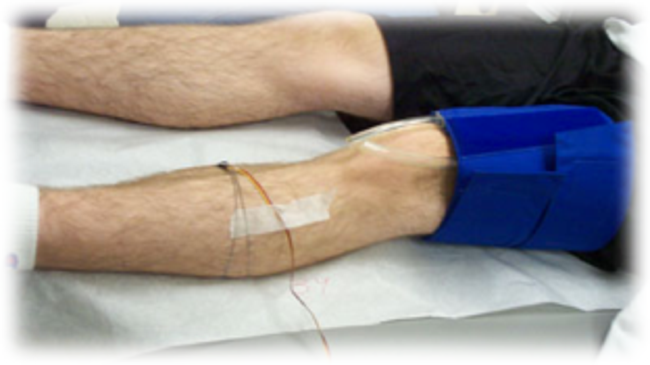
\includegraphics[width=0.75\textwidth,keepaspectratio,trim={0.5cm 0.5cm 0.5cm 0.5cm}, clip]{figure6}    
%	\caption[Strain gauge plethysmography]{Representation of a classic plethysmography waveform from the heart cycle. The image on the top represents the electrical signal of the heart. The one before is the plethysmography waveform of the circulation.}
%	\label{fig:strain gauge}
%\end{figure}


\section{Methods to measure blood flow}
The measurement of blood flow can be traced back to mid 19th century. The first experiment carried out required the use of a known volume of air in a sealed U-tube which was attached to a blood vessel to estimate the arterial blood flow using the Poiselle equation \cite{dokunin1958modification}. From there different methods were developed such as collection of venous outflow in a graduated cylinder for a establish time interval. Later on, this technique was improved using drop recorders \cite{jayanthy2011measuring}.

A long time has passed since then, and different methods have been developed to assess the rate of blood flow, which can be mildly invasive and non-invasive. More advanced methods use diagnostics imaging which provides great accuracy but not great portability for a home setting, such as Arterial-spin-labeled MRI (ASL-MRI) \cite{schmitt2003quantitative} and positron emission tomography (PET) \cite{baron1999mapping}. There is a vast number of instruments and variation of a single technique able to measure blood flow. For instance, Doppler can be implemented using light or sound waves. It also can be used as a continued monitor or diagnostics image technique. 

The following list of equipment describe the methods or instruments that can measure blood flow in an extremity. However, this list has been limited to devices that are portable, and need minimum assistance from a specialist. Diagnostic imaging techniques provide high accuracy, but they are confined to a clinical setting.

\subsection{Doppler ultrasound}
\label{section literature UD}
The Ultrasound method is widely used in medicine, which can be applied to different fields like diagnostic imaging, localising tissues and the most common blood flow measurement. The usage of this method dates back to the work of Satomura and Kaneko \cite{satomura1959study} with the development of a non-invasive method to study blood flow in the periphery. Currently, it is common to see it in medical practice when measuring the blood flow of the brachial or femoral arteries \cite{casey2008measuring} as shown in figure \ref{fig:UD Instrument}. 

\begin{figure}[!htpb]
	\centering
	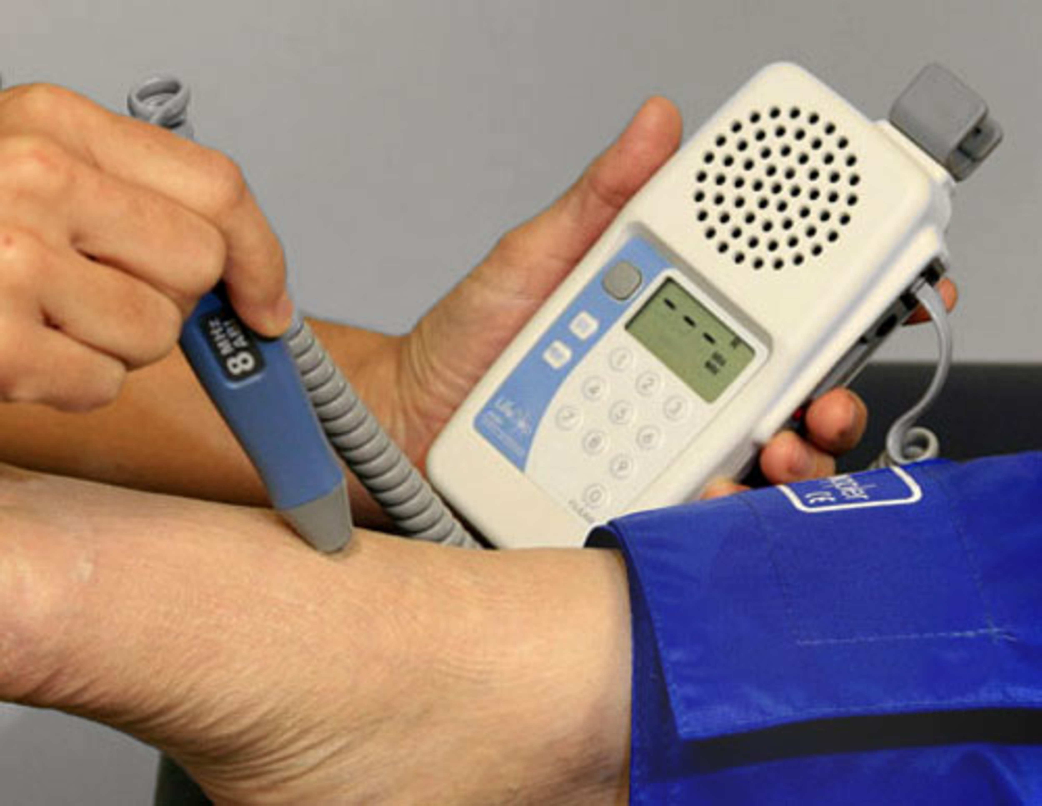
\includegraphics[width=0.65\textwidth,keepaspectratio]{ultrasound_doppler}    
	\caption[Ultrasound Doppler instrument]{Ultrasound Doppler instrument used measuring blood flow in femoral artery \cite{ultrasoundinstrument}}
	\label{fig:UD Instrument}
\end{figure}

From the technical point of view, this method operates on any wavelength above the ultrasound spectrum (above \SI{20}{\kilo\hertz}). Conventional equipment, operates in the range of \SIrange{2}{15}{\mega\hertz} \cite{jayanthy2011measuring}. Christian Doppler (1803-1853) was the first in describing the relation between the frequency of a source and its velocity relative to its source \cite{surgeonhand2002Hand}. From his studies derives the principle that takes its name the Doppler effect. 

The principle behind this technique in medicine is the propagation of ultrasound waves through the tissue. The Doppler method measures the velocity of particles in a liquid solution using the frequency shift of backscattered ultrasound \cite{orekhova2013doppler}. In other words, if an electromagnetic wave is transmitted at a fixed frequency and is reflected by a moving body, then the frequency of the received signal will be shifted (see Figure \ref{fig:Doppler method}) \cite{jayanthy2011measuring, casey2008measuring, surgeonhand2002Hand,ht:MD2}. A device under this principle can detect moving blood cells within a vessel. When an erythrocyte passes through a vessel under the electromagnetic beam a frequency shift occurs, which is proportional to the blood flow velocity \cite{gill1979pulsed}.

\begin{figure}[!htpb]
	\centering
	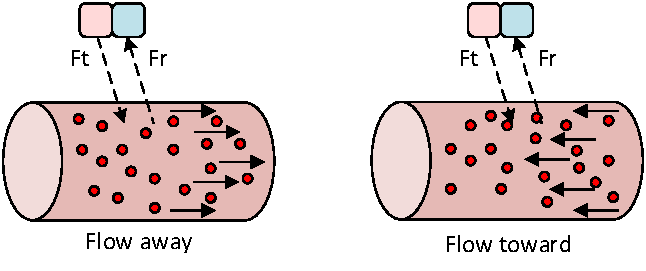
\includegraphics[width=0.65\textwidth,keepaspectratio]{figure5}    
	\caption[Doppler technique to measure flow]{Representation of the Doppler technique measuring blood flow. The cylinder represents the vessel, the red dots are the RBCs. The \textit{Ft} and \textit{Fr} are the frequencies of transmission and reception of the sensor. The phase shift between both signals change according to the movement of the particles.}
	\label{fig:Doppler method}
\end{figure}

Estimating of the blood flow based on this principle requires measuring the arterial diameter and the blood velocity. Using this parameters is possible to calculate the blood flow by multiplying the blood's mean velocity (\si{\cm \per \second}) by the cross-sectional area of the artery in \si{\square \cm}, then multiplied by \SI{60}{seconds} to express the value in millilitres per minute (\si{\milli\litre\per\minute}) \cite{casey2008measuring}. 

Some of the advantages of this method are: it is entirely non-invasive, measures velocity continuously, it is portable, consumes little energy, and can be hand-held. These features make it an excellent choice for home use. However, there is some disadvantage when measuring blood flow with this method. First, the operator requires some skill to locate the artery accurately. Some instruments provide a sound feedback that relates to the flow velocity of the artery. However, there are different levels of sound or pitch to identify the right vessel correctly. Second, it is recommended to use a low insonation angles ($\sim$ \SI{60}{\degree}) for limiting errors \cite{raadegran1999limb} which also require steady hands from the operator. Third, it is effective when the limb and the artery are in a fixed position, it is quite sensitive to motion. Last, as mentioned previously, it requires measuring the arterial diameter to convert velocity to flow. Which it is a significant disadvantage because the only way to measure this parameter accurately is by using imaging methods \cite{chapter4bloodflow} but this could be quite complicated for a home setting.

\subsection{Optical methods measuring blood flow}
\label{section literature Optic}
Light is one of the most common electromagnetic energies applied in medicine. Using optical methods is possible to estimate blood flow by measuring volume changes or by applying complex imaging techniques. One of the key features of this method is its mostly non-invasive or inclusive contact-less for some applications. Furthermore, optical imaging techniques also offer high resolution, it is cost effective when compared to MRI or PET, and is a non-ionising source \cite{jayanthy2011measuring}.

It is one of the most popular methods to monitor continuously volume changes using the principle of optical absorption of the arterial blood. In principle, it requires a coherent light source provided by a laser/light emitting diode (LED) set to a specific wavelength according to the application. The light propagates in the  due to the transport of individual photons which under the area of influence may be absorbed or scattered \cite{schmitt2003quantitative}. 

This method is so popular that is used in mostly every clinical setting and  for personal use. The latter has become widely available thanks to the use of activity monitors that utilise optical methods like the one employed in the Apple Watch \cite{culbert2017user}. So, it is clear that this method can be applied to home setting due to its versatility and portability. The following application describe the methods to used for estimation of the flow rate. 

\subsubsection{Photoplesthymography}
\label{section literature PPG}
The word plethysmography roots from the Greek word \textit{plethymos} that mean an increase in population and \textit{graphos} that is to write. In other words, it can be defined as the measurement of any volume within the human body. In medicine, some of the typical applications are the measurement of volume changes in lungs caused by the respiratory system or blood vessels caused by the circulatory system~\cite{turcott2004methods}. More specifically when referring to the latter, plethysmography aims to measures the pulsatile volume changes when the heart pumps blood in and out of a segment of the human body. 

A plethysmography device produces an output waveform that is synchronous to the heart cycle. The shape of the signal is similar to an arterial pressure waveform. In fact, the plethysmography plot represents the volume of the arterial vasculature obtaining a measure of the arterial pulse amplitude. This waveform gives meaningful information about the pulse velocity and indications of possible arterial obstruction.

This method is technically known as photoelectric plethysmography or PPG for short. Nowadays, it is one of the most popular methods used in medical applications. It is non-invasive and can use a wide range of light wavelengths to obtain a plethysmography graph. It is widely used for monitoring or evaluating heart rate, oxygen saturation, peripheral arterial pressure and peripheral microcirculation after skin grafting, drug ingestion, burns or revascularization~\cite{holohan1996plethysmography}. There are two different techniques to obtain readings. One is transmission-mode (see figure \ref{fig:PPG transmission}.) which works by placing the tissue of interest (i.e. finger, toe or ear lobe) between the light emitting diode (LED) and the photoreceptor (PD). The other is PPG reflectance-mode (see figure\ref{fig:PPG reflectance}) by placing the LED next to photoelectric cell over the surface of the tissue. PPG uses the AC component of the signal for arterial pulse detection and the DC component for venous evaluation~\cite{higgins1986photoplethysmographic}. It also uses different kinds of wavelengths to avoid interference from external sources of light. The principle behind PPG is the detection of the degree of attenuation of backscatter light from the superficial layers of skin about \SIrange{1.5}{2.0}{\milli\meter} ~\cite{holohan1996plethysmography,kim1986pulse,bashkatov2005optical}. The amount of reflected light varies with the total number of RBC’s in the cutaneous micro-circulation, which alters the wavelength during each cardiac cycle. This method provides valuable information from the waveform analysis for the initial diagnostics of peripheral arterial disease (PAD) \cite{allen1993development, williams2005evaluation, alnaeb2007optical} and chronic peripheral venous insufficiency (CVI) \cite{eberhardt2005chronic,norris1983quantitative}.


\begin{figure*}[!htbp]
	\centering
	\begin{subfigure}[t]{0.45\textwidth}
		\centering
		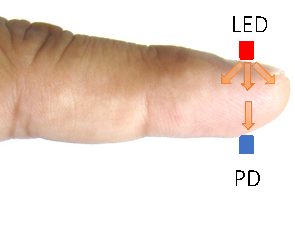
\includegraphics[height=4cm]{figure7a}
		\caption{Placement of LED and photodetector in transmission mode}
		\label{fig:PPG transmission}
	\end{subfigure}%
	~ 
	\begin{subfigure}[t]{0.45\textwidth}
		\centering
		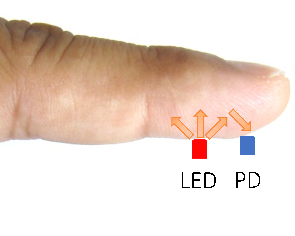
\includegraphics[height=4cm]{figure7b}
		\caption{Placement of LED and photodetector in reflectance mode}
		\label{fig:PPG reflectance}
	\end{subfigure}
	\caption[PPG sensors placemens as transmission and reflectance modes]{PPG light emitter placement and receptor according to the mode, transmission and reflectance}
	\label{fig:PPG modes}
\end{figure*}

One can say that plethysmography is not a quantitative blood flow measurement by itself but an estimation of blood concentration of a volume of tissue. Indeed, this assumption is correct, but studies have suggested that is possible to estimate blood flow when combining optical methods with other techniques. For instance, using the tissue absorption of the near-infrared spectroscopy (NIRS) is possible to estimate blood flow when combined with venous occlusion plethysmography (see section \ref{section literature VOP}) \cite{van2001performance, harel2008near, de1993noninvasive, gurley2012noninvasive}. NIRS takes the principle of the different level of absorption of oxygenated and deoxygenated haemoglobin, thus from the dynamic absorption pattern the blood flow can be determined. The study performed by Gurley et al. shows that the increase of total haemoglobin concentrations (THC) during venous occlusion can be converted from \si{\micro M  \ tHB\per\sec} to \si{\mL \ blood \per 100 \ \mL \ tissue \per\min}.

Some of the disadvantages of PPG are that only measures a small area at the time. Therefore, it is not possible to get a spatial distribution of the blood volume change over a significant portion of the skin \cite{wu2003ppgi}. Additionally, skin pigmentation has proven to be a factor of error as well as nail polish \cite{fallow2013influence}. Also, due to light's scattering in tissue is not possible to estimate its full penetration in the skin. Therefore, it is not possible to calculate the volume of tissue being measured.


\subsubsection{Laser Doppler Flowmetry}
\label{section literature LDF}
LDF is a non-invasive optical method to estimate the blood perfusion in the microcirculatory bed under the skin. This device uses the same Doppler principle described in section \ref{section literature UD}. However, as its name suggests, it uses a beam of light as the electromagnetic source. In brief, it requires a laser diode emitting a wavelength commonly between \SI{633}{\nano\metre} (red) and \SI{780}{\nano\metre} (near-infrared) with an intensity of about \SI{1}{\milli\watt} \cite{fredriksson2007laser}. A flexible fibre optic delivers and detects the light applied to a roughly \SI{1}{\cubic\mm} of tissue. After that, the light scatters by tissue and the moving blood cells. Scattering by a moving blood cell with haemoglobin produces a frequency shift, whereas scattering from stationary tissue results unshifted. The velocity of the red blood cell passing through the beam is equivalent to the frequency shift. 

Analysis of the backscattered light provides information of the blood cell velocity given by the frequency Doppler shift \cite{dirnagl1989continuous,fredriksson2007laser}, and the fraction of the backscattered light that is Doppler shifted is proportional to the total volume of moving blood cells concentrated in the tissue \cite{dirnagl1989continuous}. As a result, an index of red blood cells flow is calculated from the product of mean Doppler shift and the fraction of light that is Doppler shifted \cite{dirnagl1989continuous}. This blood perfusion index is also known as flux. Figure \ref{fig:LDF method} overviews the laser doppler flowmetry theory, more detail of the principle behind it has been described in the work of Fredriksson et al. \cite{fredriksson2007laser}.  

\begin{figure}[!htpb]
	\centering
	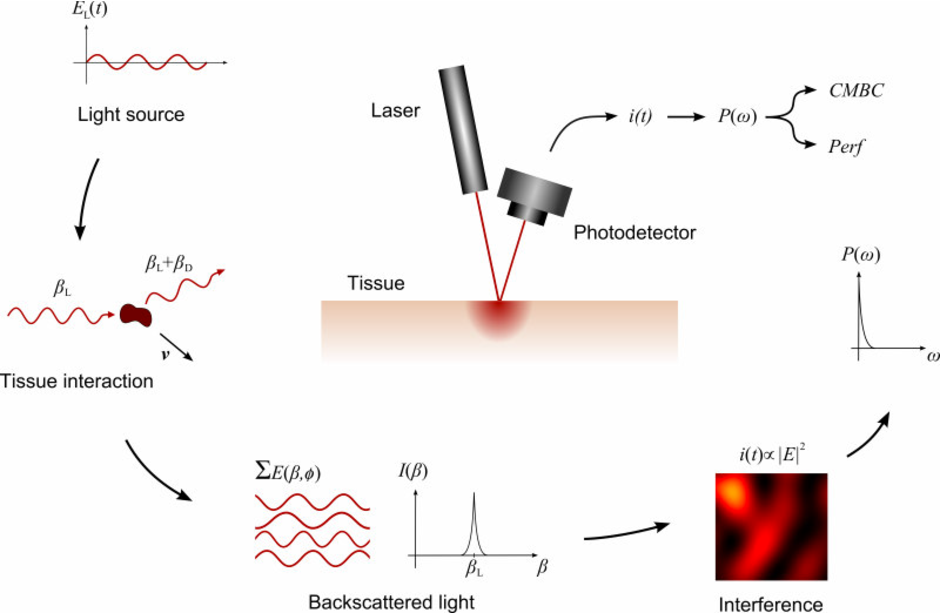
\includegraphics[width=0.8\textwidth,keepaspectratio]{LDF}    
	\caption[Laser Doppler flowmetry theory overview]{The electromagnetic wave is emitted by light $E_L(t)$, the interaction with a red blood tissue produce backscatter light $\beta_L$. The photodetector detects the light and process the frequencies of the backscattered light that produces a power spectral density $P(\omega)$ that allows to estimate the concentration of moving blood cells (CMBC) and the perfusion index (\textit{Perf}). This image has been copied from \cite{fredriksson2007laser} to explain the theory behind LDF}
	\label{fig:LDF method}
\end{figure}

Some instruments can monitor blood flow in absolute blood flow units. However, there are some doubts about this quantification because the value is based on an empirical calibration correlated to other methods \cite{cooke1990laser}. Another drawback is that the measurement is quite superficial, LDF uses a wavelength which its penetration is quite shallow. For instance, light in the wavelength of \SI{840}{\nano \metre} only penetrates up to \SI{2.5}{\milli\metre} \cite{bashkatov2005optical}, and the total volume of tissue being studies is quite small about \SI{0.1}{\cubic\mm} or less \cite{briers2013laser}. Therefore, location is a key component to get a proper measurement as an area with a good amount of capillaries equals to more blow flow distribution around the surface of the skin. Thus, more blood particles can be detected without going to deep into the tissue. 

This method has the potential to be used in a home setting; it can be portable, easy to locate and battery operated. Nonetheless, some of the critics to this method are: the measurement is affected by temperature, it is recommended to have a stable room temperature, and it is susceptible to motion artefact, the probe must be attached firmly \cite{fredriksson2007laser}. 

\subsubsection{Laser speckle contrast imaging (LSCI)}
\label{section literature LSC}
The Laser speckle laser is a fairly new technique that is still under study. Some of the medical applications of this method have on the measurement of cerebral blood flow \cite{dunn2001dynamic}, microcirculatory research \cite{domoki2012evaluation}, dentistry \cite{stoianovici2011assessment} and wound assessment \cite{stewart2005comparison} just to name some. This method can be catalogued as an imaging technique because it requires processing of images to obtain a final result. 

\begin{figure}[!htpb]
	\centering
	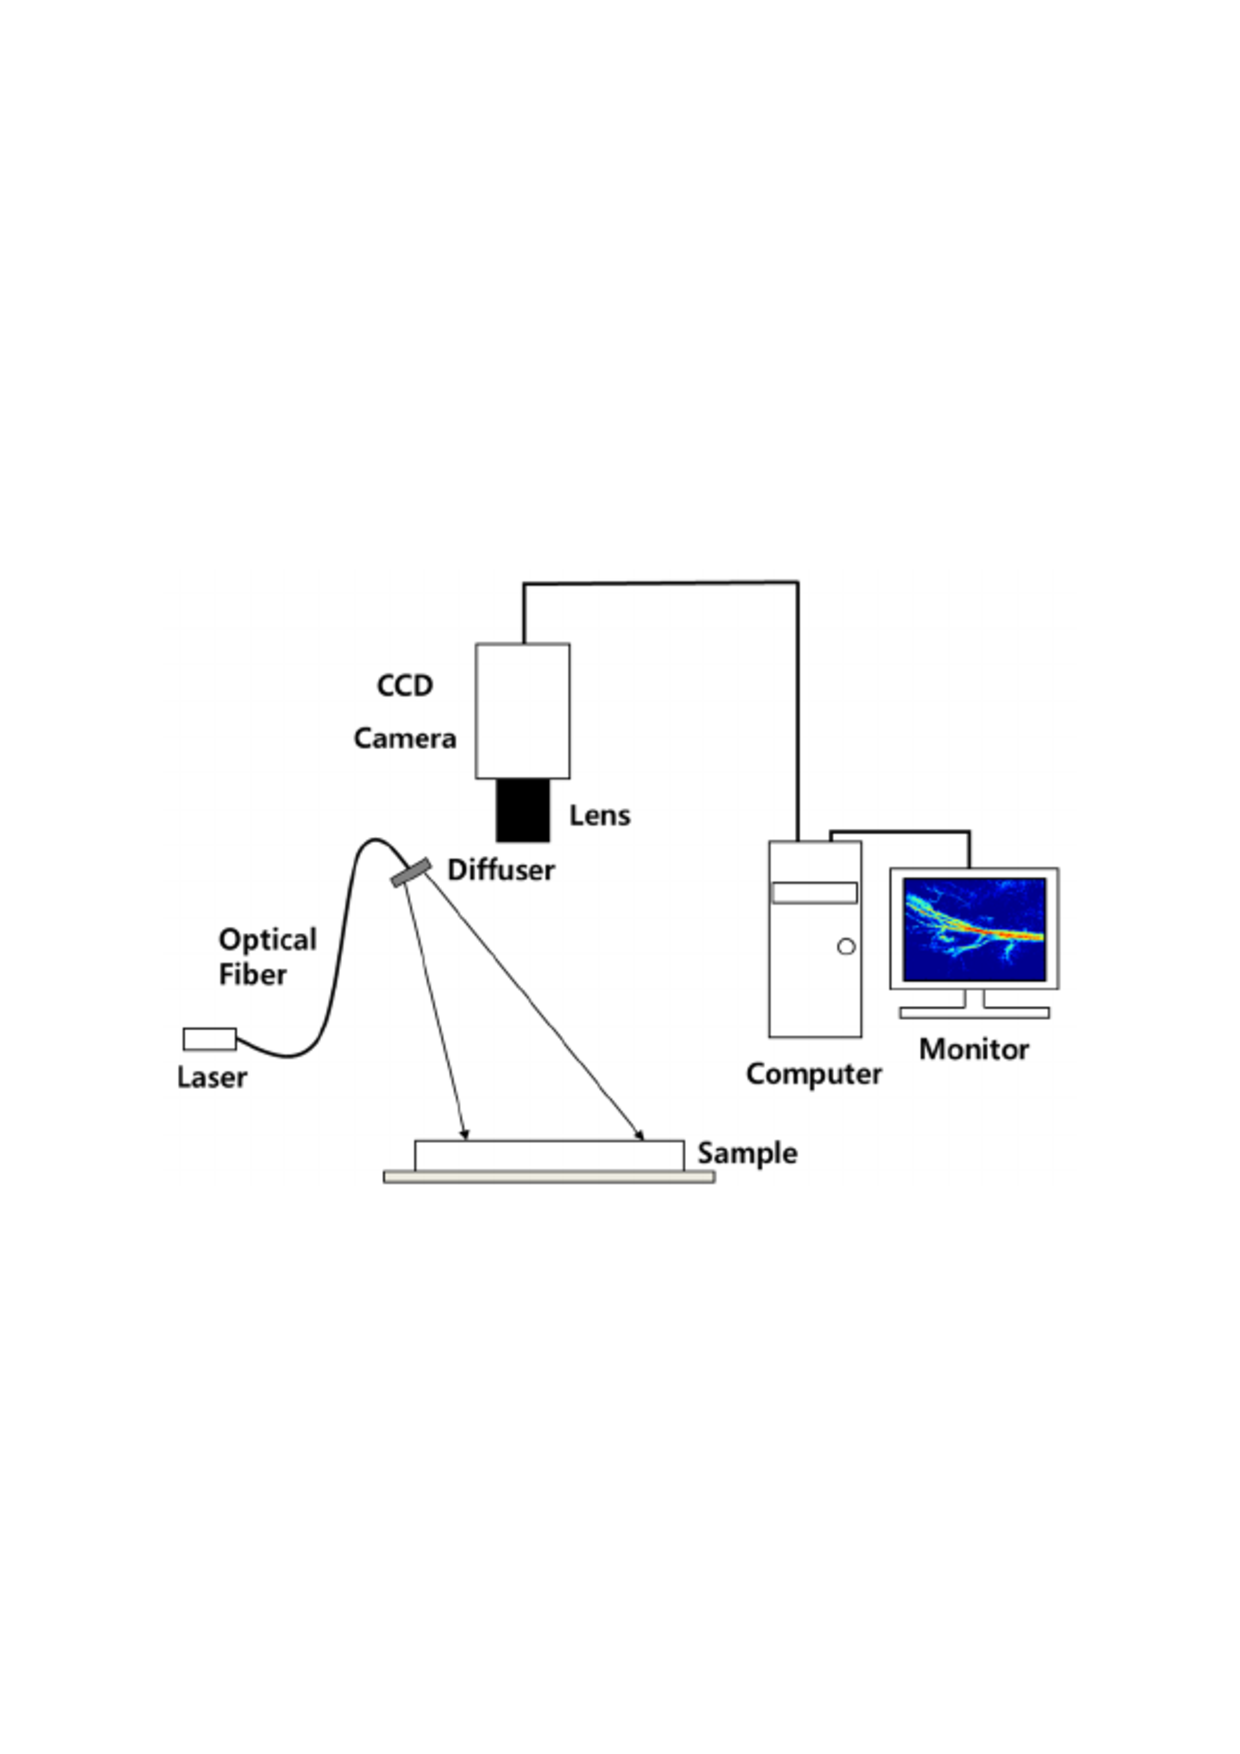
\includegraphics[width=0.8\textwidth,keepaspectratio]{lsci}    
	\caption[Setup of a Laser speckle contrast imaging]{A LSCI device requires a laser illuminating a surface, a CCD camera and a computer for the statistical analysis of the images. Image retrieved from \cite{son2013contrast}}
	\label{fig:LSCI}
\end{figure}


The set-up of a LSCI instrument is quite simple, but the processing behind it can be quite complicated. Figure \ref{fig:LSCI} shows a common experimental procedure. A coherent (laser) light beam illuminates a sample, which is recorded by a CCD (Charge Coupled Device) camera. A custom software captures the speckle pattern which a computer later process and displays as an image \cite{jayanthy2011measuring, son2013contrast, duncan2008can}. The software controls the camera's exposure time, amount of pixels, local contrast area and option of colours to code the contrast. 

Speckle images are generated by the interference pattern produced by the laser beam scattering on a rough surface, which is a random intensity distribution pattern created by the random refractive index fluctuations of the sample. This speckle pattern can only be explained by statistics \cite{goodman1975statistical}. Similar to LDF, stationary tissue produces a constant intensity contrast but scattering from moving particles like blood cells produce fluctuations in the intensity of the speckle pattern \cite{son2013contrast}. These fluctuations reduce the local speckle contrast, hence the contrast value is inversely proportional to the blood flow speed. 

LCSI has the potential of being used in a home setting. Some of the advantages of the device are: it can be portable and probably battery operated if a mobile device replaces the computer. No exogenous material is required to produce a high spatial-temporal resolution image \cite{duncan2008can}; making it completely non-invasive. The image generated is easy to understand for non-expert eyes. Thus low skills are required to operate the device. A technical improvement with Doppler techniques is that area is limited just to the focal distance of the camera, whereas Doppler targets a single point measurement. However, there are some disadvantages of this method. For instance, the image is just a representation of the surface vasculature; it is not possible to monitor large vessels blood flow. Although studies are being performed to quantify regional blood flow, this method remains as a qualitative method until the statistic behind it are better-understood \cite{duncan2008can}. 

\subsection{Venous occlusion plethysmography}
\label{section literature VOP}
Venous occlusion plethysmography (VOP) is a common method used in medicine to assess different vascular problems in humans, especially towards the limbs. It has been around for more than 100 years providing valuable information about the behaviour of the vascular endothelium in health and disease \cite{joyner2001belfast}. As its name suggests, this method uses plethysmography to evaluate the vascular response of the patient. However, estimating blood rate from this method requires to be combined with other instruments capable of measure the change of volume around a limb.

The principle behind VOP is that a pneumatic cuff is inflated around the upper-arm or tight below diastolic pressure, commonly about \SIrange{40}{50}{\mmHg}. Thus, the arterial inflow continues toward the limb whereas venous outflow is blocked \cite{joyner2001belfast, casey2008measuring}. As a result, the blood pooling effect swells the limb increasing its volume. Then, blood flow rate is calculated as linear increases of limb's volume over time which is thought to be proportional to the rate of arterial inflow \cite{joannides2006clinical, casey2008measuring}.

One could argue that having a cuff in a home setting could be cumbersome or may require assistance. However, there have been developments of portable blood pressure monitors which have simplified this approach. For instance, as shown in figure \ref{fig:nokiabpm}, the Nokia BPM+ \cite{nokiabpm} which is a wireless instrument that automates the process of obstructing the upper arm.

\begin{figure}[!htpb]
	\centering
	
\includegraphics[width=0.65\textwidth,keepaspectratio]{nokiabpm}    
	\caption[Nokia BPM+]{Portable blood pressure monitor from Nokia. Image retrieved from \cite{nokiabpm}}
	\label{fig:nokiabpm}
\end{figure}
 
Apart from the cuff, it is essential to measure plethysmographic changes around the limb for this method to estimate blood flow. A wide variety of instruments have been used in a clinical setting for estimating flow rate but just a few have the potential to be used at home. The following are some of these methods currently available.  

\subsubsection{Air/Water plethysmography}
\label{section literature air plethysmography}
Air/water plethysmography is not a common method to measure a limb’s change of volume. It has been used as an alternative or research method as explained by Chuah et al.~\cite{chuah2004plethysmography} for measurement of plethysmography without venous occlusion. This approach uses a special chamber that contains the limb in a closed area with orifices where transducers and calibration devices are connected. The arm is introduced into the case through a tight rubber sleeve to ensure that the instrument is airtight.  The plethysmography pulsations are detected by measuring the displacement of the surrounding air.water with a sensor connected to the chamber, which also moves the rubber diaphragm whereby a Doppler ultrasound transducer measures displacement. 

This method can provide quite accurate results but motion artefact causes ripples movements that affect the final value. Furthermore, this method could be burdensome for a home setting or even for surgery applications. It requires and extra participant to aid positioning the arm within the chamber and perform the adequate calibration. Also, the portability of this method is quite questionable as require too many parts in order to work.

\begin{figure}[!htpb]
	\centering
	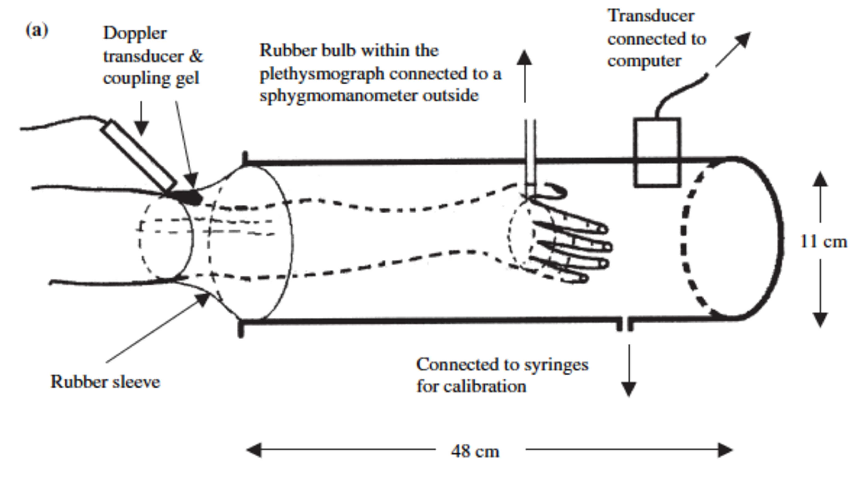
\includegraphics[width=0.8\textwidth,keepaspectratio]{figure4}    
	\caption[Air plethysmography method]{Representation of an air plethysmography device. It requires a one side open cylinder with a rubber sleeve. There is a compartment where the air displacement caused by each cardiac cycle can be measured. Image reproduces from \cite{chuah2004plethysmography}}
	\label{fig:air plethysmography}
\end{figure}

\subsubsection{Strain gauge plethysmography}
\label{section literature stain grauge}
This method also known as SGP (strain gauge plethysmography) is a non-invasive method to quantify retrograde outflow in the deep venous system and peripheral arterial disease \cite{holohan1996plethysmography}. It works by applying a strain gauge around the limb being studied. The transducer could be a tube filled in with a conductive material such as mercury and gallium and connected to a source of electricity. However, alternative methods that do not use clinically banned mercury have been developed using electrical conductive fluids \cite{flowers1981strain}. When the gauge experiences variations of circumference caused by a change of volume of the rib cage or the pulse in a limb, the resistance of the sensor varies accordingly, obtaining an electrical waveform. To increase sensitivity for venous filling measurements occlusion cuffs would be required, as shown in Figure~\ref{fig:strain gauge}. This method does not provide reliable quantitative data for venous occlusion but provides qualitative data for the function of the extremity in venous insufficiency \cite{holohan1996plethysmography}. 

This method present some advantages when used in a home setting. First, it can be portable as only one point of measurement is required. Seconds, it is non-invasive, and requires minimum skills to be used. Nonetheless, one latent problem is the use of mercury on some sensors. This is a poisonous metal which is not recommended to have at home. New electrodes can be used \cite{flowers1981strain} which could minimise this issue. Last, the instrument just measures changes of volume in a confine circumference around the sensor. That means that is not sensing changes around a large volume of tissue. 

\begin{figure}[!htpb]
	\centering
	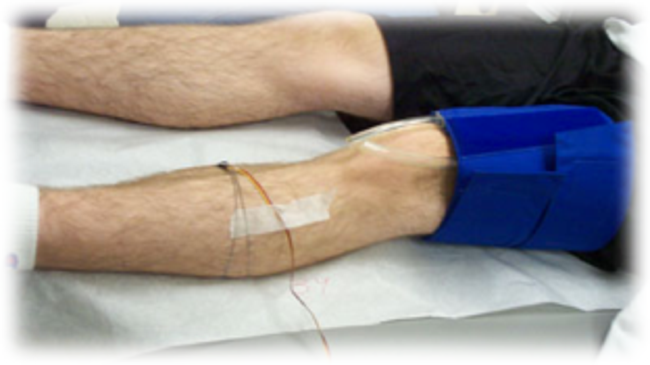
\includegraphics[width=0.75\textwidth,keepaspectratio,trim={0.5cm 0.5cm 0.5cm 0.5cm}, clip]{figure6}    
	\caption[Strain gauge plethysmography]{Representation of a classic plethysmography waveform from the heart cycle. The image on the top represents the electrical signal of the heart. The one before is the plethysmography waveform of the circulation.}
	\label{fig:strain gauge}
\end{figure}

\subsubsection{Bioelectrical Impedance plethysmography}
\label{section literature BI}
Bioelectrical impedance plethysmography is another method that measures changes in blood volume in different parts of the body, like in the thoracic cavity or limbs \cite{bera2014bioelectrical}. In principle, it senses small changes of bioelectrical impedance due to the increase of blood cells in a volume of tissue. For instance, when the heart’s systole increases blood flow, the volume of a limb rises due to the inflow of blood (swelling) \cite{martinsen2011bioimpedance}. Consequently, there are changes of impedance correlated to the small variation of volume and flow in a limb. Some medical application might require the use of pneumatic cuffs to analyse venous filling. There are several medical applications for this kind of technique such as heart stroke volume (SV) measurement, cardiac output (CO), thoracic respiratory volume, oedema and detection of deep vein thrombosis (DVT) \cite{holohan1996plethysmography}. 

Bioelectrical impedance plethysmography has been demonstrated to have a linear relation with other plethysmographic instruments, like strain gauge. For instance, the studies performed by Mohapatra~\cite{mohapatra1979measurement} and Schraibman~\cite{schraibman1975comparison} showed a significant relationship between both techniques between both techniques.

In the chapter \ref{chapter impedance} the principles of operation of this technology are described in more detail. As a brief, this method requires applying a small amount of current into the body at a specific frequency, and amplitude, usually between \SIrange{1}{500}{\kHz} \cite{kyle2004bioelectrical} and bellow \SI{5}{\mA}. Body's bioelectrical impedance is a relation between the electrical potential measured, and the electrical current applied. Commonly a set of four electrodes are placed on the surface of the skin where a pair converts the electrical conductivity into ionic conductivity and the other to sense the voltage drop. An increase in the amount of blood in a section of the body drops its total impedance. Therefore, there is a direct relation between the population of red blood cells and the impedance measurement \cite{mattern1957determination}. 

The blood flow rate can estimate from the impedance plethysmography signal. Indeed, impedance maybe regarded as a measurement of both volume and flow, a change of volume must be due to a flow \cite{martinsen2011bioimpedance}. Some studies use venous occlusion plethysmography as a method to estimate the flow rate \cite{mohapatra1979measurement, costeloe1980continuous, yamakoshi1980limb}, whereas other techniques are centred in the analysis of the plethysmographic signal without occlusion \cite{brown1975impedance, marks1985computer, porter1985measurement, corciova2011peripheral}. 

Nyober et al. \cite{nyober1950electrical} proposed the reigning equation \ref{eq:DVDT} from which blood flow is estimated. The author defined that the blood flow is proportional to the change of impedance in relation to the distance between the potential electrodes and basal impedance of the tissue. The section \ref{section procedure Z to V and Q} describes more in detail the equation required to convert impedance into the blood flow.

Calculating blood flow from the impedance signal can be applicable for home use, these are some of the advantages. First of all is non-invasive as just requires four electrodes for measurement. Additionally, the device uses low-energy, the current required to read impedance is below \SI{5}{\mA} which can be obtained with a battery operated instrument. Furthermore, the tissue's volume being monitored is more substantial than other techniques as the boundary of the measurement is limited by the position of the potential electrodes. In fact, whole body measurements can be achieved as described in free-fat measurements performed by Kyle et al. \cite{kyle2004bioelectrical}. IPG is less affected by temperature \cite{bera2014bioelectrical}. It provides more data than single point measurements as helps to assess venous blood volume and arterial pulsations \cite{bera2014bioelectrical}. Some of the disadvantages of this technique is that like all the methods is sensitive to motion. Electric current is required for measurement, thus is not suitable for a certain population, and finally, there is an electrode-skin impedance error when there is no full contact. 
 
\section{Conclusion}
This section introduces the circulatory system starting from blood cells and its functionality. It is important to remark the importance of blood cells in transporting nutrients and oxygen whole tissue around the body. The blood vessels structure was explained as well as the way how blood can reach every cell in the body, and the interchange of nutrients and by-products. The cardiac cycle showed how heart operates as a pump and how blood flows in and out of it. The anatomy of the upper extremities will serve as a reference when advancing further in this document.  

Illnesses and problems due to poor circulation towards the periphery were described, and it explained why is essential to monitored blood flow in a home setting \rvmynote{I need to add this in the section about circulation}. Then different instruments were shown with the potential to quantify blood flow a home environment; the Doppler Ultrasound method was described, as well as various optical instruments. The venous occlusion plethysmography is a useful tool for quantifying blood rate. Three different apparatuses have the potential to be used at home. However, obtaining the flow rate from the bioelectrical impedance plethysmography seems to be an excellent choice because it assesses a large volume of tissue compared to other methods. 


%********************************** %Nomenclatures in chapter  **************************************
\nomenclature[z-Hb]{Hb}{Haemoglobin}
\nomenclature[z-ATP]{ATP}{Adenosine Triphosphate}
\nomenclature[z-rbc]{RBC}{Red Blood Cells}
\nomenclature[z-abi]{ABI}{Ankle-Brachial index}
\nomenclature[z-wbc]{WBC}{White Blood Cells}
\nomenclature[z-PVD]{PVD}{Peripheral vascular disease}
\nomenclature[z-bia]{BIA}{Bioelectrical impedance analysis}
\nomenclature[z-DFI]{DFI}{Doppler flowmetry}
\nomenclature[z-DVT]{DVT}{Deep vein thrombosis}
\nomenclature[z-cli]{CLI}{Critical Limb Ischemia}
\nomenclature[z-PAD]{PAD}{Peripheral Arterial Disease}
\nomenclature[z-SV]{SV}{Strove Volume}
\nomenclature[z-LED]{LED}{Light emitting diode}
\nomenclature[z-CVI]{CVI}{Chronic peripheral venous insufficiency}
\nomenclature[z-ppg]{PPG}{Photoplethysmography}
\nomenclature[z-ipg]{iPG}{Impedance Plethysmography}
\nomenclature[z-CO]{CO}{Cardiac output}
\nomenclature[z-SGP]{SGP}{strain gauge plethysmography}
\nomenclature[z-BIA]{BIA}{Bioelectrical impedance analysis}
\nomenclature[z-NIRS]{NIRS}{Near-infrared spectroscopy}
\nomenclature[z-LSCI]{LSCI}{Laser speckle contrast imaging}
\nomenclature[z-CCD]{CCD}{Charge Coupled Device}


%\nomenclature[z-cif]{$CIF$}{Cauchy's Integral Formula}                                % first letter Z is for Acronyms 
%\nomenclature[a-F]{$F$}{complex function}                                                   % first letter A is for Roman symbols
%\nomenclature[g-p]{$\pi$}{ $\simeq 3.14\ldots$}                                             % first letter G is for Greek Symbols
%\nomenclature[g-i]{$\iota$}{unit imaginary number $\sqrt{-1}$}                      % first letter G is for Greek Symbols
%\nomenclature[g-g]{$\gamma$}{a simply closed curve on a complex plane}  % first letter G is for Greek Symbols
%\nomenclature[x-i]{$\oint_\gamma$}{integration around a curve $\gamma$} % first letter X is for Other Symbols
%\nomenclature[r-j]{$j$}{superscript index}                                                       % first letter R is for superscripts
%\nomenclature[s-0]{$0$}{subscript index}                                                        % first letter S is for subscriptsd
